\documentclass[10pt,driverfallback=hypertex]{report}
\usepackage{amsmath}
\usepackage{graphicx}
\usepackage{ifthen}
\usepackage{math}
\usepackage{multirow} 
\usepackage{ode}

\definecolor{heavyblue}{cmyk}{1,1,0,0.25}

\hypersetup{
  pdftitle=Lab Notes for Math 201: DEs for Engineers,
  pdfpagemode=UseOutlines,
  citebordercolor=0 0 1,
  colorlinks=true,
  allcolors=heavyblue,
  breaklinks=true,
  pdfauthor={Malcolm Roberts and Samantha Marion},
  pdfpagetransition=Dissolve,
  bookmarks=true
}

\newcounter{showsolutions}
\setcounter{showsolutions}{0}
\newcounter{small}
\setcounter{small}{0}


%\usepackage[pdftitle={Lab Manual for Math 201 DEs for Geers}]{hyperref}
%\usepackage[driverfallback=hypertex,pdftitle={Lab Manual for Math 201 DEs for Geers},pdfauthor={Malcolm Roberts and Samantha Marion}]{hyperref}

\ifthenelse{\value{small}=1}{
  \usepackage[paperwidth=9.1cm, paperheight=11cm, hmargin={0.17in, 0.17in}, vmargin={0.50in, 0.17in}]{geometry}
}{}
%\usepackage[paper size={90mm, 120mm},left=2mm,right=2mm,top=2mm,bottom=2mm,nohead]{geometry}
%\usepackage[letterpaper,textheight=8.5in,textwidth=6in,dvips]{geometry}



\begin{document}
\sloppy



%%
%% title page
%%

\pagestyle{empty}
\ifthenelse{\value{small}=0}{
  \begin{center}
    \ \vspace{1in}
    
    \textsf{\LARGE Math 201} \\
    \vspace{0.2in}
    \textsf{\LARGE Differential Equations for Engineers}
    \vspace{2in}
    
    \textsf{\Huge an \emph{unofficial} lab manual}
    \vspace{2.5in}
    
    by Malcolm Roberts and Samantha Marion
    \vspace{0.5in}
}{ % small-format title page:
  \begin{center}
    \ \vspace{0.5cm}
    
    \textsf{\LARGE Math 201:} \\
    \vspace{1cm}
    \textsf{\LARGE Differential Equations for Engineers}
    \vspace{2cm}
    
    \textsf{\Large an \emph{unofficial} lab manual}
    \vspace{2cm}
    
    by Malcolm Roberts and Samantha Marion
    \vspace{0.2cm}
}


%  \textsf{\Large by GAME (Graduates at Alberta Mathematics Etc.)}
\end{center}

%%
%% disclaimer and copyright page
%%
\newpage

\ \vspace{5in}

\noindent
This (unofficial) manual was prepared for \emph{Graduates at Alberta
  Mathematics Etc.} (GAME) by Malcolm Roberts and Samantha Marion.
\vspace{0.5in}

\noindent
This manual is not officially endorsed by the University of
Alberta or the Department of Mathematical and Statistical Sciences at
the University of Alberta.
\vspace{0.5in}

\noindent
Copyright 2009, Graduates at Alberta Mathematics Etc.  All rights
reserved.

%%
%% the rest of the manual...
%%

\newpage
\pagestyle{plain}
\pagenumbering{arabic}

\section*{Introduction}

Differential equations (abbreviated DEs) are equations involving functions and
their derivatives. For example,
\begin{dmath}
  \label{eg1}
  \dd{y}{x} =y
\end{dmath}
is a differential equation. In this case, $y$ is a function of the independent
variable $x$, and we would like to determine $y$. The solution to this
equation is
\begin{dmath*}
  y = Ce^x,
\end{dmath*}
with $C$ an arbitrary constant, since 
\begin{dmath*}\dd{y}{x}=\dd{}{x}Ce^x=Ce^x=y.\end{dmath*} 
That is, if we
plug $y=Ce^x$ into equation~\eqref{eg1}, both sides match. If we modify this
a little bit, say letting $y=Ce^x +x$, then the left hand side doesn't
match the right:
\begin{dmath*}
  \dd{y}{x} = \dd{}{x}(Ce^x +x) 
  = Ce^x + 1 = y +1 
  \neq y,
\end{dmath*}
so it isn't a solution to equation~\eqref{eg1}.

An initial value problem (abbreviated as IVP) is a differential equation
combined with one or more initial conditions. For example,
\begin{dmath*}[compact]
  \dd{y}{x}=y, \qquad y(0)=1
\end{dmath*}
is an initial value problem.
The differential equation is solved by $y=Ce^x$, for any value of $C$. However,
the only way to satisfy 
\begin{dmath*}
  y(0)=1
\end{dmath*}
with the solution $y=Ce^x$ is to set $C=1$. That is, the solution to
the initial value problem is 
\begin{dmath*}
  y=e^x,
\end{dmath*}
since it satisfies both the differential equation and the initial
conditions.

Differential equations are extremely useful for modelling complex behaviour in
most sciences. Unfortunately, we do not know how to solve most
differential equations analytically, and in practice we often have to
make approximations when dealing with real systems. However, when we can solve
DEs analytically, we should, and understanding how to solve simple DEs will
help to understand the properties of solutions of more complicated problems.



\chapter{Separable and Exact DEs}
\ifthenelse{\value{small}=1}{\newpage}

\section{Separable equations}

Separable equations are differential equations of the form
\begin{dmath}
  \label{separable}
  \boxed{h(y) \dd{y}{x} = g(x)}.
\end{dmath}
These are simple to solve: from equation~\eqref{separable}, we can
just split the derivative and integrate: $ h(y)\, dy = g(x) \, dx$
becomes
\begin{dmath*}
  \boxed{  \int h(y) \, dy = \int g(x) \, dx},
\end{dmath*}
and then all we need to do is find the integral and solve for $y$.\\

\noindent\emph{Example}: Consider the equation
\begin{dmath}
  \label{separableexample}
  y \dd{y}{x} = \sin(x)
\end{dmath}
with initial condition $ y(0) = 1$. Separating and integrating,
\begin{dmath*}
  \int y \, dy = \int \sin(x) \, dx,
\end{dmath*}
yields
\begin{dmath*}
  \frac{y^2}{2} = -\cos(x) + C
\end{dmath*}
where $C$ is a constant that will be determined by the initial conditions.
Let us now solve for $y$:
\begin{dmath*}
  y(x) = \pm \sqrt{2 C -2 \cos(x)}.
\end{dmath*}
Notice that we have two different solutions a positive one and a negative on.
 We can use the initial condition $y(0)=1$ to eliminate one. Since
\begin{dmath*}
  y(0) = \pm  \sqrt{2 C - 2 \cos(0) } = \pm \sqrt{2C-2} =1,
\end{dmath*}
and $1$ is positive, we must choose the positive root.
Thus,
\begin{dmath*}
  \(C-1\)^2 =1/2
\end{dmath*}
so
\begin{dmath*}
  C=3/2,
\end{dmath*}
and the solution is
\begin{dmath*}
  y(x) = \sqrt{3 - 2\cos(x)}.
\end{dmath*}

It's a good idea to check that the solution that you got is correct. This is
pretty easy; just plug the solution into the original equation. From
the above example, $y(x) = \sqrt{3 - 2\cos(x)}$, so
\begin{dmath*}
  \dd{y}{x} = \frac{\sin(x)}{\sqrt{3 -2 \cos(x)}}.
\end{dmath*}
Putting this into the left-hand side of
equation~\eqref{separableexample} yields
\begin{dmath*}
  y \dd{y}{x}=
  \(\sqrt{3 - 2\cos(x)}\) \times \(\frac{\sin(x)}{\sqrt{3 -2 \cos(x)}}\)
  = \sin(x),
\end{dmath*}
which matches the right-hand side of
equation~\eqref{separableexample}, and we can be sure that we got the
correct answer. \qed



\section{Exact Equations}

\begin{definition}\emph{Exact equations.}
  Homogeneous first-order differential equations can be written in the form
  $M(x,y) dx + N(x,y)dy=0.$ If
  \begin{dmath*}
    \boxed{\pp{M(x,y)}{y} =   \pp{N(x,y)}{x}}
    \end{dmath*}
  then the equation is called \emph{exact}.
\end{definition}
The nice thing with exact differentials is that Poincare's lemma implies
the existence of a function $F$ such that $dF = M(x,y)dx + N(x,y)dy$, and
$dF$, called the differential of $F$, can be thought of as ``how much $F$
changes''. Since $dF=0$, $F$ does not change, i.e.\ it's constant.
Solutions to the exact differential equation are given
implicitly by $F(x,y)=\text{constant}$.

Exact equations are straightforward to solve: after a little bit of trickery,
we simply integrate. Let
\begin{dmath}
  \label{exactsol}
  \boxed{  F(x,y) = \int M(x,y)\, dx + g(y) }.
\end{dmath}
We require that $\pp{}{y}F(x,y)= N(x,y)$, which will allow us to determine
$g(y)$. That is,
\begin{dmath*}
  \pp{F(x,y)}{y}
  = \pp{}{y}\(\int M(x,y) \, dx + g(y)\)
  = \int \pp{M(x,y)}{y} \, dx + \pp{g(y)}{y}
  = N(x,y) + g'(y).
\end{dmath*}
This tells us what $g'(y)$ is, so we now know $g(y)$ up to some constant
$C$. We can put this into equation~\eqref{exactsol}, which gives us the
implicit solution
\begin{dmath}
  \label{exactimpl}
  \boxed{F(x,y) =C }.
\end{dmath}
In many cases, we can solve for $y$, thus getting an explicit solution
$y=f(x)$ so that $F(x,f(x))=C$, but sometimes all we have for a solution
is something in the form of equation~\eqref{exactimpl}.\\

\noindent\emph{Example}: Solve
\begin{dmath*}
  y\, dx + \(y^2 + x \) dy =0
\end{dmath*}
Using the notation above, we have $M(x,y)=y$, and $N(x,y)=y^2 +x$.
This equation is exact, since
\begin{dmath*}[compact]
  \dd{}{y}y = 1 = \dd{\(y^2 +x\)}{x}.
\end{dmath*}
So write
\begin{dmath*}
  F(x,y)
  = \int y \, dx + g(y)
  = xy + g(y).
\end{dmath*}
We now need to set $\pp{}{y} F = N$, so
\begin{dmath*}
  \pp{}{y}\[xy + g(y)\] = y^2 +x
\end{dmath*}
which implies that $g'(y) = y^2$. We integrate this to get
\begin{dmath}
  \label{exactC1}
  g(y) = \frac{y^3}{3} + C.
\end{dmath}
The solution is then given by
\begin{dmath}
  \label{exactC2}
  F(x,y) = xy + \frac{y^3}{3} 
  \no
  =C. \qed
\end{dmath}
(Note that in the above equation we have played fast and loose with
the undetermined constant $C$; in fact, $C$ changed sign between
equation~\eqref{exactC1} and equation~\eqref{exactC2}. We perform this
abuse of notation because $C$ is \emph{undetermined}, so there's not
much point nailing it down to a value until the very last moment.)

\section{Problems}

\begin{enumerate}
\item
  Does $y = \sqrt{3-2\sin x}$ solve the differential equation
  \begin{dmath*}
    y\frac{dy}{dx}=\sin(x)?
  \end{dmath*}

\item
  Solve the equation
  \begin{dmath*}
    (2xy + 3) dx + (x^2 - 1) dy = 0
  \end{dmath*}
  \hidesolution{This is an exact equation}

\item
  Solve the logistic map $\dd{y}{x} = y - y^2$ as a separable equation.

\item
  Give the general solution to the differential equation
  \begin{dmath*}
    \ddt{y} = 1 + \frac{1}{y^2}
  \end{dmath*}
  \hidesolution{
    This is a separable equation:
    \begin{dmath*}[compact]
      \frac{dy}{1+\frac{1}{y^2}} = dt
      \implies
      \int dt = \int  \frac{dy}{1+\frac{1}{y^2}}
    \end{dmath*}
    But, since
    \begin{dmath*}
      \frac{1}{1+\frac{1}{y^2}} 
      = \frac{y^2}{y^2+1} 
      = 1 - \frac{1}{1+y^2}
    \end{dmath*}
    so
    \begin{dmath*}
      t 
      = \int  \(1 - \frac{1}{1+y^2}\) dy 
      = y + \arctan y + C,
    \end{dmath*}
    which implicitly defines $y(t)$.
  }

\end{enumerate}



\chapter{Linear Equations \& Transformations}
\newpage

\section{Linear Equations}

Linear equations have the form
\begin{dmath}
  \label{linear}
  \boxed{\dd{y}{x} + P(x) y = Q(x)}.
\end{dmath}
To solve these equations, we use an \emph{integrating factor}. That is, if
we define the integrating factor $\mu$ as
\begin{dmath*}
  \boxed{\mu(x) \doteq \exp\[ \int P(x)\, dx \]},
\end{dmath*}
then notice that
\begin{dmath*}
  \dd{}{x}\(\mu y \) 
  = \dd{\mu}{x} y + \mu \dd{y}{x}
  = \mu P(x) y + \mu \dd{y}{x}.
\end{dmath*}
So if we multiply equation~\eqref{linear} by $\mu$, we get
\begin{dmath*}
  \dd{}{x}\(\mu y \) = \mu Q,
\end{dmath*}
which we can now solve by taking the integral of both sides with respect to
$x$. Doing this, we get
\begin{dmath*}
  d\(\mu y\) = \mu Q \, dx
\end{dmath*}
which implies that
\begin{dmath*}
  \mu y = \int \mu Q \, dx + C .
\end{dmath*}
This provides us with the general formula for the integrating factor, 
\begin{dmath}
  \label{linearf}
  \boxed{y = \frac{\int \mu Q \, dx + C}{\mu}.}
\end{dmath}
\\

\noindent \emph{Example}:
\label{linearsec}
Consider the equation
\begin{dmath*}
  \dd{y}{x} + \frac{y}{x} = 2 e^x.
\end{dmath*}
We identify $P(x)=1/x$ and $Q(x)=2e^x$. The integrating factor is
\begin{dmath*}
  \mu(x) = \mbox{exp}\[\int \frac{1}{x} \, dx \] = e^{\ln x} = x.
\end{dmath*}
Then,
\begin{dmath}
  \label{linearex}
  \dd{}{x} \(x y \) = 2 x e^x,
\end{dmath}
integrating this gives
\begin{dmath}
  x y = \int 2 x e^x \, dx.
\end{dmath}
From the formula (equation~\eqref{linearf}), we have
\begin{dmath}
  \label{linearexx}
  y = \frac{\int \mu Q \, dx + C}{\mu} = \frac{\int 2 x e^x \, dx + C}{x}.
\end{dmath}
To solve this, we use integration by parts. That is,
$\int u \, dv = uv - \int v\,  du$. We choose $u=x$ and $dv = e^x \, dx$, so
$du = dx$, and $v=e^x$. Thus,
\begin{dmath*}
  \int x e^x \,dx 
  = x e^x + \int e^x \,dx 
  = x e^x + e^x.
\end{dmath*}
Putting this into equation~\eqref{linearexx} yields
\begin{dmath*}
  y = 2 e^x \(1 + \frac{1}{x}\) + \frac{C}{x}. \qed
\end{dmath*}
If we had been provided with initial conditions, we would now use them
to determine the value of $C$.


% TODO: show how they can check this?



\section{Equations that can be solved via substitution}

Sometimes it is possible to make a substitution to transform a
differential equation into something that we already know how to
solve.  For example, the integrating factor technique transforms
linear equations into separable equations. This can be a very powerful
technique. Unfortunately, each type of equation needs its own
particular substitution and this makes substitution not as straight
forward as other techniques. 

The most important examples of substitution are linear, homogeneous,
and Bernoulli equations. We also consider two other types of equations
that can be solved by substitution, which are shown in the flow chart in
Figure~\ref{fig:first_order_flow_shar}.

\subsubsection{Homogeneous Equations}
\begin{dmath*}
  \boxed{\dd{y}{x} = f\(\frac{y}{x}\)}.
\end{dmath*}
We solve this by substituting $v=y/x$, so that
\begin{dmath*}[compact]
  \dd{y}{x} = v + x \dd{v}{x},
  \quad \implies \quad
  v + x \dd{v}{x} = f(v),
\end{dmath*}
which can be written as the separable equation
\begin{dmath*}
\boxed{\dd{v}{x} = \frac{f(v) -v}{x}}.
\end{dmath*}

\noindent \emph{Example}:
\begin{dmath*}[compact]
  \dd{y}{x} = \frac{x}{y}, \mbox{ with } y(1) = 2.
\end{dmath*}
This is homogeneous, so let $v=y/x$, and then $f(v) = \frac{1}{v}$, so
\begin{dmath*}
  v + x \dd{v}{x} = \frac{1}{v}.
\end{dmath*}
The equation is now separable:
\begin{dmath*}
  \frac{1}{\frac{1}{v} -v} \, dv = \frac{1}{x}\, dx.
\end{dmath*}
Integrating both sides gives
\begin{dmath*}
  \int \frac{v}{1-v^2}dv = \int \frac{1}{x} \, dx.
\end{dmath*}
Let $u = 1-v^2$ to solve the integral:
\begin{dmath*}
  -\frac{1}{2} \int \frac{1}{u}du = \ln x+ \ln C
\end{dmath*}
which implies that
\begin{dmath*}
  \ln\(u\)=\ln\(1-v^2 \) = \ln \frac{C}{x^2}.
\end{dmath*}
In terms of $v$, we have
which implies that
\begin{dmath*}
  v = \pm \sqrt{1 - \frac{C}{x^2}}.
\end{dmath*}
Expressing this in terms of the original variable $y$ gives
\begin{dmath*}
  y = \pm x \sqrt{1 - \frac{C}{x^2}}.
\end{dmath*}
The initial condition is $y(1)=2$, so we choose the positive root, and
find $C$ by setting $x=1$, $y=2$, i.e.\
\begin{dmath*}
  2 = 1 \times \sqrt{1-C}
\end{dmath*}
so $C=-3$. The solution of the initial value problem is 
\begin{dmath*}
  y = x \sqrt{1 + \frac{3}{x^2}}.
\end{dmath*}

This would be a good one to check. Note that
\begin{dmath*}[compact]
  \dd{y}{x} 
  = \sqrt{1+\frac{3}{x^2}} - \frac{3/x^2}{\sqrt{1+\frac{3}{x^2}}}
  = \frac{1}{\sqrt{1+\frac{3}{x^2}}}
  = \frac{x}{y},
\end{dmath*}
so the solution is correct. \qed

\subsubsection{Bernoulli Equations}
Bernoulli equations are differential equations of the form
\begin{dmath*}
  \boxed{  \dd{y}{x} + P(x) y = Q(x)y^n}
\end{dmath*}
where $n$ can be an integer or a rational number. Note that if
$n=0$ or $n=1$, then this is just a linear equation.

We solve this by substituting $v=y^{1-n}$, so that
\begin{dmath*}[compact]
  \dd{v}{x} = \(1-n\)y^{-n}\dd{y}{x}
\end{dmath*}
and rearranging gives
\begin{dmath*}
  \frac{1}{1-n} \dd{v}{x} + P(x)v = Q(x).
\end{dmath*}
We can write this as a linear equation:
\begin{dmath*}
  \boxed{\dd{v}{x} + (1-n)P(x)v = (1-n)Q(x).}
\end{dmath*}

\noindent\emph{Example}:
\begin{dmath*}
  \dd{y}{x} -\half \frac{y}{x} = -e^x y^3
\end{dmath*}
Since $n=3$, choose $v=y^{-2}$. Then
\begin{dmath*}[compact]
  \dd{v}{x} = -2 y^{-3} \dd{y}{x}
  \quad \implies \quad
  \dd{v}{x} = -2 y^{-3}\( \half \frac{y}{x}  - e^x y^3\)
  \quad \implies \quad
  \dd{v}{x} + \frac{v}{x} = 2 e^x,
\end{dmath*}
which is the linear equation given as the example from section \ref{linearsec}.
\qed


%\subsubsection{Equations with Linear Coefficients}
% Question: doesn't case 1 follow from case 2?
% Sam's answer: Yes, I believe it does
%\be
%\(a_1 x + b_1 y + c_1\)dx +2 \(a_2 x + b_2 y + c_2\)dy =0
%\ee
%We deal with equations where $a_1 b_2 \neq a_2 b_1$, for which there
%are two cases:
%\begin{enumerate}
%\item if $c_1=c_2=0$, then
%\be
%\dd{y}{x} = -\frac{a_1 + b_1 \(y/x\)}{a_2+ b_2 \(y/x\)},
%\ee
%which is homogeneous.
%\item if either $c_1$ or $c_2$ is not zero, then we use the substitution
%$x=u+h$ and $y=v+k$, with $h$ and $k$ constants which obey the relationship
%\be
%a_1h + b_1 k + c_1 &=&0 \\ \nonumber
%a_2h + b_2 k + c_2 &=&0 .
%\ee
%This reduces the problem to
%\be
%\dd{v}{u} = -\frac{a_1 + b_1 \(v/u\)}{a_2 + b_2 \(v/u\)},
%\ee
%which is homogeneous in $u$ and $v$.
%\end{enumerate}


\newpage
\subsection{Flow chart for solving first-order DEs}

As we have seen, it is sometimes necessary to use several
transformations in order to solve a given DE.  Each type of first
order DE that we have seen so far is ultimately separable, as outlined
in the flow chart below, or exact.

%FIXME: refer to this somewhere
\vspace{0.5in}
\begin{figure}[htbp]
  \centering
  \ifthenelse{\value{small}=0}{
    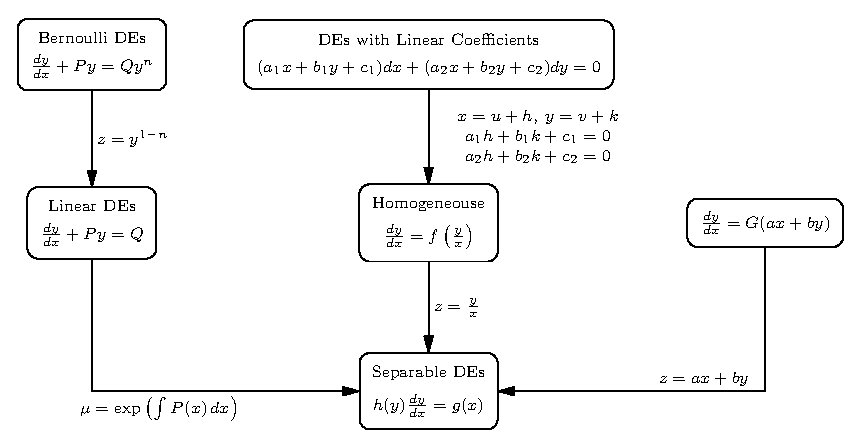
\includegraphics{figures/firstorderchart}
  }{
    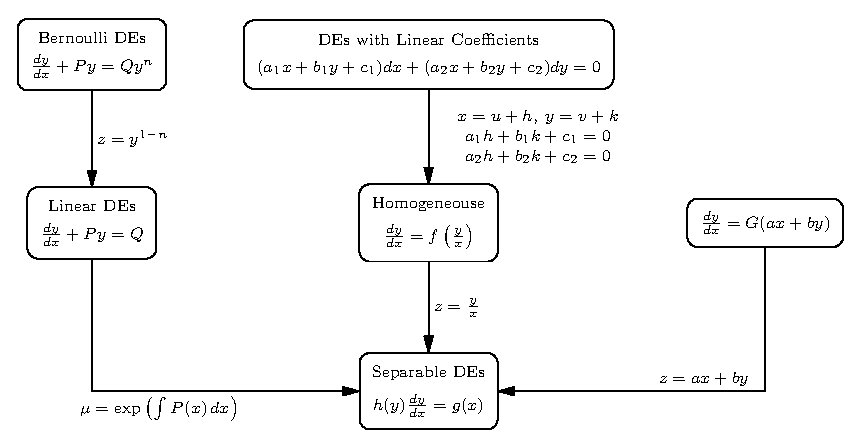
\includegraphics[width=\textwidth]{figures/firstorderchart}
  }
  \caption{Flow chart for solving first-order DEs}
  \label{fig:first_order_flow_shar}
\end{figure}


\section{Problems}

\begin{enumerate}

\item
% a linear equation
Solve the initial value problem
\begin{dmath*}
  (x^2 + 1) \frac{dy}{dx} + 4xy = 4x,
\end{dmath*}
with initial condition
\begin{dmath*}
  y(0) =\ 0\ \text{ or }\ 1\ 
\end{dmath*}
(choose one, and circle your choice).
\hidesolution{Rewrite this equation as
  \begin{dmath*}
    \frac{dy}{dx} + \frac{4x}{x^2+1}y = \frac{4x}{x^2+1}
  \end{dmath*}
  which is linear with $P(x) = \frac{4x}{x^2+1}$, so let
  \begin{dmath*}
    \mu(x) = \exp \left(\int P(x)\, dx \right)
    = \exp \left( \int \frac{4x}{x^2+1} \, dx \right) = \exp(2 \ln (x^2+1))
    = \exp(\ln (x^2+1)^2) = (x^2+1)^2.
  \end{dmath*}
(Note that we can omit the absolute value bars around $x^2+1$ since it is
always positive.) Then multiplying through by $\mu(x)$ we obtain
\begin{dmath*}
  (x+1)^2 \frac{dy}{dx} + 4x(x^2+1)y 
  = 4x(x^2+1) 
\end{dmath*}
\begin{dmath*}
  \frac{d}{dx} \left( (x^2+1)y \right) 
  = 4x^3+4x.
\end{dmath*}
Integrating yields
\begin{dmath*}
  (x^2+1)^2 y 
  = x^4 + 2x^2 + C 
\end{dmath*}
\begin{dmath*}
  y = \frac{x^4 + 2x^2 + C}{(x^2+1)^2}.
\end{dmath*}
Solving the IVP $y(0) = 1$ gives $C = 1$, then the solution is
\begin{dmath*}
  y = \frac{x^4 + 2x^2 + 1}{(x^2+1)^2} 
  = \frac{(x^2+1)^2}{(x^2+1)^2} 
  \equiv 1.
\end{dmath*}
It's actually obvious from just looking at the problem that $y \equiv 1$ is a
solution to this IVP, so you could just have wrote it down and quoted the
result that linear equations have unique solutions to IVPs.

This equation is also separable since we may rewrite it as
\begin{dmath*}
  (x^2+1) \frac{dy}{dx}
  = 4x(1-y) \qquad\Rightarrow\qquad \frac{1}{1-y} \frac{dy}{dx}
  = \frac{4x}{x^2+1}
\end{dmath*}
but in dividing by $1-y$ we have destroyed the solution $y \equiv 1$,
which is the (unique) solution to the initial value problem $y(0) =
1$, so it is not possible to solve the IVP $y(0) = 1$ by separating
this equation.  This is why I let you choose instead the IVP $y(0) =
0$, which has solution
\begin{dmath*}
  y = 1 - \frac{1}{(x^2+1)^2}
\end{dmath*}
}

\item
 Joe headed out to the bar in his new Thinsulate jacket, but drank
too much and passed out on the way home. Ignoring the heat that his body
produces, his temperature is determined by Newton's law of cooling.
Determine Joe's temperature $T$ at time $t$ by solving Newton's law of cooling,
both as a separation problem and a linear problem
\begin{dmath*}
  \dd{T}{t} = -r\(T - T_{\text{env}}\),
\end{dmath*}
where $T(0)=37$, $T_{\text{env}}=-40$, and $r=5$ (Thinsulate's r-value).
\hidesolution{TODO: write solution.}

\item
Solve the logistic map,
\begin{dmath*}
  \dd{y}{x} = y - y^2.
\end{dmath*}
as a Bernoulli equation
\hidesolution{TODO: write solution.}

\item
Solve the differential equation
\begin{dmath*}
  \dd{y}{x} = \frac{y}{x} + x^2y^2.
\end{dmath*}
\hidesolution{TODO: write solution. Bernoulli equation.}

\item
  Equations of the form $\dd{y}{x} = f(ax+by)$ may be transformed into a
  separable equation via the substitution  $v=ax + by$. Using this technique,
  solve the differential equation
  \begin{dmath*}
    \dd{y}{x} = - \(4x -y\)^2
  \end{dmath*}
  \hidesolution{
    Let $v=4x-y$, so $y'=4-v'$. Then
    \begin{dmath*}
      v' = v^2 +4 = (v-2)(v+2),
    \end{dmath*}
    which is separable. That is, $\frac{dv}{(v-2)(v+2)} = dx$, so, using
    partial fractions,
    \begin{dmath*}
      \int \frac{1/4}{v-2} -\frac{1/4}{v+2} \, dv
      = \frac{1}{4} \ln\abs{v-2} - \frac{1}{4} \ln\abs{v+2} = x + C.
    \end{dmath*}
    Substituting $v=4x-y$ back in, we get the implicit solution
    \begin{dmath*}
      \ln\abs{\frac{4x-y-2}{4x-y+2}} = 4x +C.
    \end{dmath*}
    Solving for $y$ yields
    \begin{dmath*}
      y = \frac{Ce^{4x}\(4x+2\) -4x +2}{1-Ce^{4x}}.
    \end{dmath*}
  }

\item
  Equations of the form
  \begin{dmath*}
    \(a_1 x + b_1 y + c_1\)dx +\(a_2 x + b_2 y + c_2\)dy =0
  \end{dmath*}
  can be transformed into homogeneous equations by using the substitution
  $x=u+h$ and $y=v+k$, with $h$ and $k$ constants which obey the relationship
  \bee
  a_1h + b_1 k + c_1 &=&0 \\
  a_2h + b_2 k + c_2 &=&0 .
  \eee
  This reduces the problem to
  \begin{dmath*}
    \dd{v}{u} = -\frac{a_1 + b_1 \(v/u\)}{a_2 + b_2 \(v/u\)},
  \end{dmath*}
  which is homogeneous in $u$ and $v$.
  Solve the differential equation
  \begin{dmath*}
    \(2y + 2\) dx + \(x +y+2\) dy=0
  \end{dmath*}
  using this technique.



  \item
    Solve the following differential equation:
    \begin{dmath*}
    \dd{y}{x} = \frac{y}{x} + x^2 y^2
    \end{dmath*}
    \hidesolution{
      This is a Bernoulli equation with $n=2$, so set $v=y^{1-n}=y^{-1}$. Then,
      \begin{dmath*}
      \dd{y}{x} = \frac{-1}{x^2}\dd{v}{x}.
      \end{dmath*}
      Then,
      \begin{dmath*}[compact]
      \frac{-1}{v^2}v' - \frac{1}{xv} = \frac{x^2}{v^2}
      \implies
      v' = \frac{v}{x} - x^2
      \end{dmath*}
      Now, let $w=v/x$, which implies that
      \begin{dmath*}
        w + x \dd{w}{x} = w -x^2 \implies \dd{w}{x} = -x^2
      \end{dmath*}
      Thus, $w = - \half x^2 + C$, so
      \begin{dmath*}[compact]
        w=\frac{v}{x} 
        = \frac{1}{xy} \implies \frac{1}{y} = \frac{-x^3}{2} + Cx
        \implies y = \frac{1}{-x^3/2 + Cx}.
      \end{dmath*}
    }

\end{enumerate}



\chapter{Second-order Linear Equations}
\ifthenelse{\value{small}=1}{\newpage}

\newcommand\ycomb{\alpha y_1 + \beta y_2}

% Text chapter 4.2
Let $a,b,c$ be real numbers. Second order equations of the form
\begin{dmath} 
  \label{sec2hom}
  a \ddtwo{y}{t} + b \dd{y}{t} + cy =0
\end{dmath}
are linear in $y$. If both $y_1$ and $y_2$ are solutions to
equation~\eqref{sec2hom}, and $\alpha$ and $\beta$ are constants, then
$$\ycomb$$
is a linear combination of $y_1$ and $y_2$. If we put this linear combination 
into the original differential equation, we get:
\begin{dmath*}
   a \ddtwo{\(\ycomb\)}{t} + b \dd{\(\ycomb\)}{t} + c \(\ycomb \)
   = \alpha\(a \ddtwo{y_1}{t} + b \dd{y_1}{t} + cy_1 \)
   +\beta\(a \ddtwo{y_2}{t} + b \dd{y_2}{t} + cy_2 \)
   = \alpha \times 0 +\beta \times 0 =0.
\end{dmath*}
In other words, $\ycomb$, which is a linear combination of $y_1$ and $y_2$, is
also a solution to equation~\eqref{sec2hom}. Being able to use this linearity
is a powerful tool that we can use to solve this very important type of
differential equation. We will, in general, have two solutions to these
second-order differential equations, and we will need two initial values to
fully determine the solution. This is expressed in the following theorem:

\begin{theorem}
  Let $b$, $c$, $Y_0$, and $Y_1 \in \mathbb{R}$.
  Then, the initial value problem
  \begin{dmath*}[compact]
    y'' + by' + cy =0, \qquad y(0)=Y_0, \quad y'(0)=Y_1
  \end{dmath*}
  has a unique solution.
\end{theorem}

\section{Homogeneous Linear Equations}
The behaviour of these systems is basically exponential. To see this,
set $y=e^{rt}$. Then, putting this into equation (\ref{sec2hom}), we get
\begin{dmath*}
  a r^2 e^{rt} + b r e^{rt} + ce^{rt}
  = e^{rt} \( ar^2 + br + c\) =0.
\end{dmath*}
Since $e^{rt}$ is never zero, there is no harm in dividing by it. This leaves
us with the \emph{characteristic equation},
\begin{dmath*}
  \boxed{ar^2 + br + c =0},
\end{dmath*}
which allows us to determine $r$ using the quadratic formula. In this way
we get two solutions,
\begin{dmath*}
  \boxed{y_1=e^{r_1 t}\text{ and }y_2=e^{r_2 t}},
\end{dmath*}
from the two solutions $r_1$ and $r_2$ of the characteristic equation.\\

\noindent\emph{Example}: Solve the second-order homogeneous equation
\begin{dmath*}
  \ddtwo{y}{t} - y =0,
\end{dmath*}
with initial conditions $y(0) =1, \, y'(0) =0.$\\
\noindent\emph{Solution}:
Setting $y=e^{rt}$, this becomes
\begin{dmath*}
  e^{rt} \(r^2 -1 \) 
  = e^{rt} \(r-1\)\(r+1\) 
  =0,
\end{dmath*}
so $r_1=-1$, and $r_2=1$. Thus,
\begin{dmath*}[compact]
  y_1(t) 
  = e^{-t}, \qquad y_2(t) 
  =e^t.
\end{dmath*}
The solution $y$ is therefore a linear combination of $y_1$ and $y_2$. That is,
\begin{dmath*}
  y(t) 
  = \alpha y_1(t) + \beta y_2(t) 
  = \alpha e^{-t} + \beta e^t,
\end{dmath*}
for some constants $\alpha$ and $\beta$ that are determined by the initial
conditions. Since $y(0)=1$,
\begin{dmath}
  \label{sec2ab1}
  y(0) = \alpha +\beta =1.
\end{dmath}
Since $y'(0)=0$, and $y'(t) = -\alpha e^{-t} + \beta e^t$,
\begin{dmath}
  \label{sec2ab2}
  y'(0) = -\alpha + \beta =0.
\end{dmath}
Combining equations~\eqref{sec2ab1} and~\eqref{sec2ab2}, it is easy to see
that $\alpha = \beta =\half$. The solution is therefore
\begin{dmath*}
y = \frac{e^{-t} + e^t}{2}. \qed
\end{dmath*}

\section{Dealing with complex roots}
%Text section 4.3
So far, we've seen only problems where the roots of the characteristic
equation are real. Of course, this isn't always the case, but we can deal with
this using \emph{Euler's Formula},
\begin{dmath*}
  \boxed{e^{i\theta} = \cos(\theta) + i \sin(\theta)}.
\end{dmath*}
For example, if we get $r_{1,2}= 4\pm 2i$, then solutions are a linear
combination of
\begin{dmath*}
  e^{(4+2i)t}
  =e^{4t}e^{i2t}
  =e^{4t} \(\cos(2t) + i \sin(2t)\)
\end{dmath*}
and
\begin{dmath*}
e^{(4-2i)t}=e^{4t}e^{-i2t}=e^{4t} \(\cos(2t) - i \sin(2t)\).
\end{dmath*}
An easy way to get all linear combinations is to just set
$$
  y_1(t) = e^{4t} \cos(2t), \qquad y_2(t) = e^{4t} \sin(2t).
$$

\noindent\emph{Example}: Give the general solution to
\begin{dmath*}
  \ddtwo{y}{t} + 1 =0
\end{dmath*}
with initial conditions $y(0) =1, \, y'(0) =0.$\\
\noindent\emph{Solution}:
The characteristic equation is
\begin{dmath*}[compact]
  r^2 +1 =0 \quad \implies \quad r = \pm i.
\end{dmath*}
The solution is then a linear combination of
\begin{dmath*}[compact]
  y_1(t) = e^{0t}\cos(t) = \cos(t), \qquad
  y_2(t) = e^{0t}\sin(t) = \sin(t)
\end{dmath*}
Setting $y(t)=\alpha \cos(t) + \beta \sin(t)$, we can input the initial
conditions to get
\bee
y(0) &=& \alpha\cos(0) + \beta\sin(0) = \alpha =1,
\\
y'(0) &=& -\alpha\sin(0) + \beta\cos(0) =\beta =0.
\eee
The solution to the IVP is then $y(t) = \cos(t)$. \qed

\section{Dealing with repeated roots}
In the above section, we were lucky, since we had two independent roots.
Two independent roots gave two independent solutions $y_1$ and $y_2$, which
we used to solve the two initial values for the problem. When we have
repeated roots, we still need to make sure that we have two independent
solutions. How do we get this? Well, just multiply one solution by $t$.
% TODO: add a footnote as to why this makes sense.

For example, suppose that we solved the characteristic equation and got
$r_1=r_2=r$. We still get one solution out of this, namely
\begin{dmath*}
  y_1(t) =e^{rt}.
\end{dmath*}
To get the second solution, just take
\begin{dmath*}
  y_2(t) = t y_1(t) = t e^{rt}.
\end{dmath*}
This works since $\ddtwo{t}{t}=0$, so the extra $t$ in $y_2$ is eventually
killed, and everything cancels out nicely.
\\

\noindent\emph{Example}: Give the general solution to
\begin{dmath*}
  \ddtwo{y}{t} - 2 \dd{y}{t}+1 =0
\end{dmath*}
with initial conditions $y(0) =1, \, y'(0) =0.$\\
\noindent\emph{Solution}:
The characteristic equation for this problem is
\begin{dmath*}
  r^2 - 2r +1 = (r-1)(r-1) =0,
\end{dmath*}
which has the double root $r_1=r_2=1$. Thus, set
$y_1(t) = e^t$ and $y_2=t e^t$, so
\begin{dmath*}
  y = \alpha e^t + \beta t e^t
\end{dmath*}
Now,
\begin{dmath*}[compact]
  y(0) = \alpha = 1.
\end{dmath*}
For the second condition, calculate that
$y'(t) = \alpha e^t + \beta e^t + \beta te^t$. Thus
\begin{dmath*}[compact]
  y'(0) = \alpha + \beta =0.
\end{dmath*}
Thus, $\alpha=1$ and $\beta =-1$, so the solution is
\begin{dmath*}[compact]
  y(t) = e^t - te^t. \qed
\end{dmath*}

\newpage
\subsection{Flow chart for $2^{\text{nd}}$-order linear homogeneous DEs}

\ifthenelse{\value{small}=0}{ 
  Second-order linear differential equations with real-valued
  coefficients will produce two (possibly equal) real roots or a pair
  of complex roots.  In this case, you will never encounter repeated
  complex roots, and you can use the following flow-chart to solve
  these types of equations:

  %FIXME: refer to this somewhere
  \vspace{0.5in}
  \begin{figure}[!h]
    \centering
    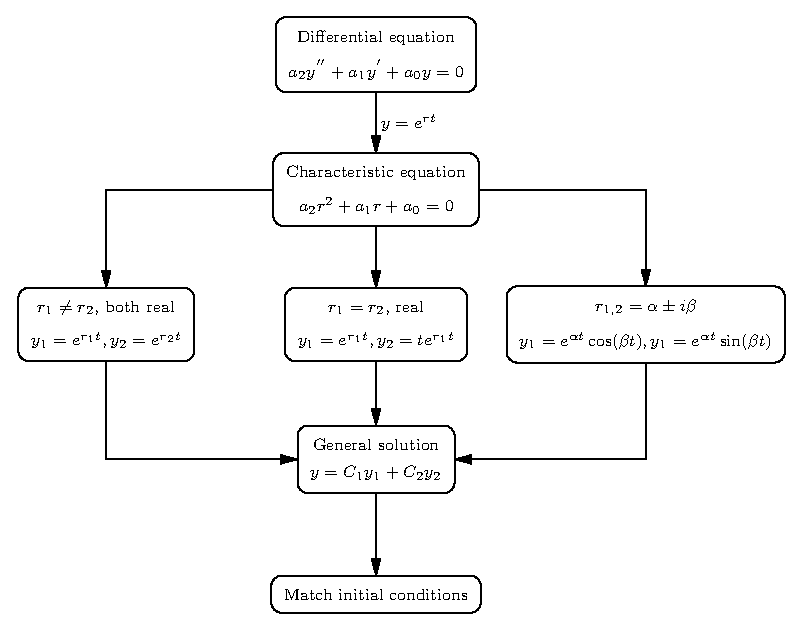
\includegraphics[width=\textwidth]{figures/linhomflow}
    \caption{Flow chart for solving second-order homogeneous DEs}
    \label{fig:linhomflow}
  \end{figure}
}{ %smaller formatting:
  \vspace{0.5in}
  \begin{figure}[!h]
    \centering
    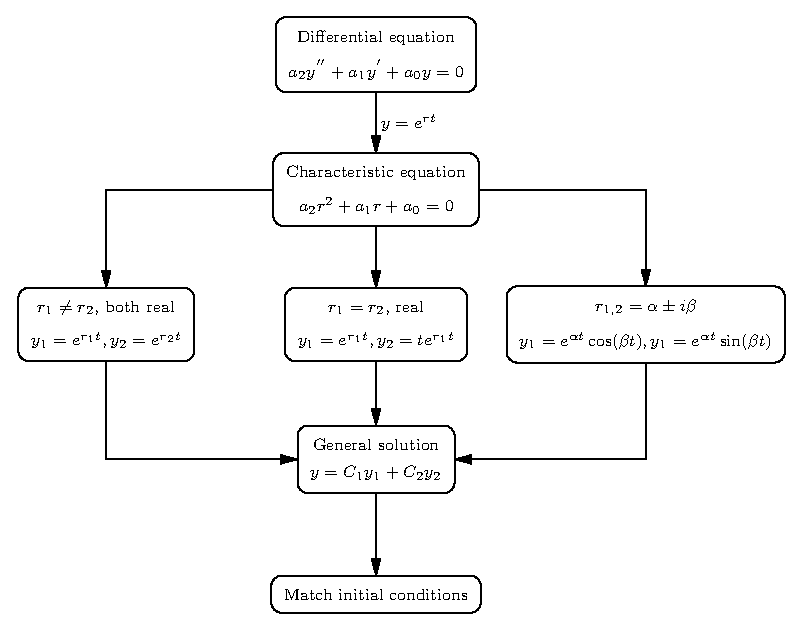
\includegraphics[width=0.9\textwidth]{figures/linhomflow}
    \caption{Flow chart for solving second-order homogeneous DEs}
    \label{fig:linhomflow}
  \end{figure}
}


\section{Problems}

\begin{enumerate}

\item
  % Real roots
  Solve the IVP
  \begin{dmath*}
    2 y'' + 5y' + 2y =0
  \end{dmath*}
  with initial conditions $y(0)=0$ and $y'(0)=3/2$.

\item
  Solve the IVP
  % imaginary roots
  \begin{dmath*}
    2 y'' + 8y =0
  \end{dmath*}
  with initial conditions $y(0)=1$ and $y'(0)=2$.

\item
  Solve the IVP
  % complex roots
  \begin{dmath*}
    y'' + 2y' + 4y=0
  \end{dmath*}
  with initial conditions $y(0)=0$ and $y'(0)=2$.
  %r = -1 \pm i \sqrt{3}
  % y =2 \sqrt{3} e^{-t} \sin(\sqrt{3}t\)

\item
  Prove Euler's formula using differential equations. \\
  Consider the IVP
  \begin{dmath*}[compact]
    y'' +y =0, \qquad y(0)=1, \quad y'(0)=i.
  \end{dmath*}
  \begin{itemize}
    \item Step 1: Show that $\{y_1=\cos(t),y_2=\sin(t)\}$ are solutions
      to the differential equation. Find a solution $y=\alpha y_1 + \beta y_2$
      to the IVP.
    \item Step 2: Using the characteristic equation, find a different pair
      of solutions $\{y_1,y_2\}$ made up of complex exponentials. Find a
      solution $y=\alpha y_1 + \beta y_2$ to the IVP.
    \item Step 3: Use the uniqueness theorem to show that these two
      solutions must be identical, thereby proving Euler's formula.
  \end{itemize}

\item
  % Mazowita's question. Solution is tex'd.
  Find the general solution of the differential equation
  \begin{dmath*}
  10, \! 000 \, y'' - 100, \! 000 \, y' + 250, \! 000 \, y = 0.
  \end{dmath*}


\item
  % Mazowita's question. Solution is tex'd.
  Solve the IVP
  \begin{dmath*}
    y'' + 4y' + 5y = 0
  \end{dmath*}
  with $y(\pi) =\ e^{-\pi},$ $y' (0) = \sqrt{\pi} + 2e^\pi$.

\end{enumerate}


\chapter{Non-homogeneous $2^{\text{nd}}$ Order Linear DEs}
\ifthenelse{\value{small}=1}{\newpage}

\section{Method of Undetermined Coefficients}
% Text section  4.4
The next step is to add a function to the right-hand side of
equation~\eqref{sec2hom}, so that we get
\begin{dmath*}
  a y'' + b y' + cy =f(t).
\end{dmath*}
Then what we have is a \emph{non-homogeneous equation} and we say that
equation $a y'' + b y' + cy =0$ is the corresponding homogeneous
equation.

In this section, we are going to restrict ourselves to a couple of
choices for $f(t)$ so that we can use the method of \emph{undetermined
  coefficients}, also known as \emph{we can probably guess what the
  answer is, so let's do that}.

The idea behind this method is trying to find the particular solution $y_p$,
which has the property
\begin{dmath} 
  \label{yp}
  a y_p'' + b y_p' + cy_p =f(t),
\end{dmath}
though it need not match the initial conditions. For instance, if
$f(t)=\sin(t)$, guessing that $y_p = A \sin(t) + B \cos(t)$ would probably do
the trick. We can just substitute $y_p = A \sin(t) + B \cos(t)$ into equation~\eqref{yp} in order to find the values of $A$ and $B$ that work.

Here is a table that will guide you, young Jedi:
%FIXME: table is too wide

\ifthenelse{\value{small}=0}{
$$
\begin{tabular}{ l |  l }
  $f(t)$ & $y_p$  \\
  \hline
  $ke^{at}$ & $Ce^{at}$  \\
  $kt^n$ & $C_n t^n + C_{n-1}t^{n-1} + \dots + C_1 t + C_0 $  \\
  $k \cos(at)$ or $k \sin(at)$ & $K \cos(at) + M\sin(at)$ \\
  $kt^n e^{at}$ & $e^{at}\(C_n t^n + C_{n-1}t^{n-1} + \dots + C_1 t + C_0\)$ \\
  $k t^n \cos(at)$ or $k t^n \sin(at)$ &
  $\(C_nt^n + \dots +C_0 \)\cos(at) + \(D_nt^n + \dots + D_0 \)\sin(at)$ \\
  $ke^{at} \cos(bt)$ or $ke^{at} \sin(bt)$ &
  $e^{at}\(K \cos(at) + M\sin(at)\)$ \\
  $k t^n e^{at }\cos(bt)$ or $k t^n e^{at} \sin(bt)$ &
  $\(C_nt^n + \dots +C_0 \)e^{at}\cos(bt)
  + \(D_nt^n \no{+} \dots + D_0 \)e^{bt}\sin(bt)$ \\
\end{tabular}
$$
}{
  % small-format
\begin{center}
  $f(t) \rightarrow y_p$:\\
  \vspace{0.3cm}
  $ke^{at} \rightarrow Ce^{at}$  \\
  \vspace{0.1cm}
  $kt^n \rightarrow  \sum_{i=0}^n C_i t^i $  \\
  \vspace{0.1cm}
  $k \sin \(at\) \rightarrow  K \cos(at) + M\sin(at)$ \\
  \vspace{0.1cm}
  $k \cos \(at\) \rightarrow  K \cos(at) + M\sin(at)$ \\
  \vspace{0.1cm}
  $kt^n e^{at} \rightarrow  e^{at}  \sum_{i=0}^n C_i t^i $ \\
  \vspace{0.1cm}
  $k t^n \cos(at) \rightarrow   \cos(at)\sum_{i=0}^n C_i t^i  +  \sin(at)\sum_{i=0}^n D_i t^i$ \\  
  \vspace{0.1cm}
  $k t^n \sin(at) \rightarrow   \cos(at)\sum_{i=0}^n C_i t^i  +  \sin(at)\sum_{i=0}^n D_i t^i$ \\
  \vspace{0.1cm}
  $ke^{at} \cos(bt) \rightarrow e^{at}\[K \cos(at) + M\sin(at)\]$ \\
  \vspace{0.1cm}
  $ke^{at} \sin(bt) \rightarrow e^{at}\[K \cos(at) + M\sin(at)\]$ \\
  \vspace{0.1cm}
  $k t^n e^{at }\cos(bt) \rightarrow
  e^{at}\cos(bt) \sum_{i=0}^n C_i t^i 
  + e^{bt}\sin(bt) \sum_{i=0}^n D_i t^i $ \\
  \vspace{0.1cm}
  $k t^n e^{at }\sin(bt) \rightarrow
  e^{at}\cos(bt) \sum_{i=0}^n C_i t^i 
  + e^{bt}\sin(bt)\sum_{i=0}^n D_i t^i $ \\
\end{center}
}
Finally, if your guess ends up being a polynomial times a linear
combination of the solutions to the corresponding homogeneous equation
(known as $y_1$ and $y_2$ in previous lab), then multiply your guess
by $t$ until it isn't. For example, if 
$$y_1=e^t, \quad y_2=e^{2t}, \quad\text{and}\quad f(t)=t^2e^t,$$ 
then you would choose 
$$y_p = t\(C_2 t^2 + C_1 t + C_0\)e^t.$$  
If 
$y_1=e^t, \quad y_2=t e^t\quad  \text{and}\quad f(t)=t^2e^t,$ then you would
choose 
$$y_p = t^2 \(C_2 t^2 + C_1 t + C_0 \)e^t.$$
\\

Once you have determined $y_p$, combine it with the homogeneous
solutions to give the general solution
\begin{dmath*}
  \boxed{y(t) = \alpha y_1(t) + \beta y_2(t) + y_p(t) }
\end{dmath*}
to match the initial conditions.
\\

\noindent \emph{Example}:
Solve the IVP
\begin{dmath} 
  \label{undetceg}
  y'' -3y' +2 y = t
\end{dmath}
with $y(0) = 3/4$ and $y'(0) = 3/2$.\\
\noindent \emph{Solution}:
This has characteristic equation
\begin{dmath*}[compact]
  r^2 -3r +2 = (r-1)(r-2) \quad \implies \quad r_1=1, \, r_2=2,
\end{dmath*}
so the homogeneous solutions are $y_1(t) = e^t, \, y_2=e^{2t}$. Since
$f(t)=t$ is not a linear combination of $y_1$ and $y_2$, we can just
choose $y_p = C_1 t + C_0$. Putting this into
equation~\eqref{undetceg}, we get
\begin{dmath*}
  \ddtwo{(C_1 t + C_0)}{t} -3\dd{(C_1 t + C_0)}{t} + 2 \(C_1 t + C_0\) =t
\end{dmath*}
which implies that
\begin{dmath*}
  -3 C_1 + 2C_1 t + 2C_0 = t,
\end{dmath*}
so $C_1=1/2$ and $C_0=3/4$. Thus, $y_p = \frac{t}{2} +\frac{3}{4}$, and the
general solution is
\begin{dmath*}
  y = \alpha e^t + \beta e^{2t} + \frac{t}{2} +\frac{3}{4}.
\end{dmath*}
Now, we satisfy the initial conditions:
\begin{dmath*}[compact]
  y(0) = \alpha + \beta +\frac{3}{4} = \frac{3}{4}
  \quad \implies \quad \alpha+\beta=0,
\end{dmath*}
and
\begin{dmath*}[compact]
y'(0) = \alpha + 2\beta + \half = \frac{3}{2}
\quad \implies \quad \alpha+2 \beta=1
\end{dmath*}
so $\alpha=-1$ and $\beta =1$. The solution is therefore
\begin{dmath*}
  y(t) = -e^t +e^{2t}  + \frac{t}{2} +\frac{3}{4}.
\end{dmath*}
Let's check this solution. We have
\bee
y(t) &=& -e^t +e^{2t}  + \frac{t}{2} +\frac{3}{4}
\\
y'(t) &=& -e^t +2e^{2t}  + \frac{1}{2}
\\
y''(t) &=& -e^t +4 e^{2t}.
\eee
Putting these into equation~\eqref{undetceg} yields
\begin{dmath*}
  y'' - 3 y' + 2 y
  = \(-e^t + 4 e^{2t}\)
  -3 \(-e^t +2e^{2t}  + \frac{1}{2} \)
  +2 \(-e^t +e^{2t}  + \frac{t}{2} + \frac{3}{4} \) 
  = t,
\end{dmath*}
as required. \qed

\section{Superposition Principle}
Suppose that we know the solution $y_{1,p}$ to
\begin{dmath*}
  ay'' + by' + cy = f(t)
\end{dmath*}
and the solution $y_{2,p}$ to
\begin{dmath*}
  ay'' + by' + cy = g(t).
\end{dmath*}
We can use these to determine the solution to the more difficult problem
\begin{dmath}
  \label{super}
  ay'' + by' +cy = A f(t) + B g(t)
\end{dmath}
by using the fact that the differential operator
\begin{dmath*}
  L = a \ddtwo{}{t}  + b \dd{}{t} + c
\end{dmath*}
is linear. That is, for constants $\alpha$ and $\beta$
\begin{dmath*}
  L\(\alpha y_{1,p} + \beta y_{2,p} \)
  =
  a \(\alpha y_{1,p} + \beta y_{2,p} \)'' + b \(\alpha y_{1,p}+\beta y_{2,p}\)'
  + c\(\alpha y_{1,p} + \beta y_{2,p} \)
  = \alpha \(a y_{1,p}'' + b y_{1,p}' + c  y_{1,p}\)
  + \beta \(a y_{2,p}'' + b y_{2,p}' + c  y_{2,p}\)
  =
  \alpha L\( y_{1,p}\)  + \beta L\(y_{2,p} \),
\end{dmath*}
just like ``linearity'' is defined in linear algebra. Then since
$L\(y_{1,p}\)= f(t)$ and $L\(y_{2,p}\) = g(t)$,
\begin{dmath*}
  L\(A y_{1,p} + B y_{2,p} \) = A f(t) + B g(t),
\end{dmath*}
which gives us the particular solution for equation~\eqref{super}
without having to do a lot of extra work.  \\

\noindent\emph{Example}: Find the general solution to
\begin{dmath*}
  y'' -3 y' -4y = t + 10 e^{-t}.
\end{dmath*}
\noindent\emph{Solution}:
The characteristic equation for the homogeneous part is
$0 = r^2 -3r -4 = (r+1)(r-4)$ which gives $r_1=-1$ and $r_2=4$. The solution
space is then spanned by $\{y_1=e^{-t},y_2=e^{4t}\}$.
We can use the superposition principle to break
this problem up into two smaller problems:
\begin{enumerate}
\item
  \begin{dmath}
    \label{supereg1}
    y'' -3 y' -4y = t
  \end{dmath}
  Notice that $t$ is not a multiple of $y_1$ or $y_2$, so, looking at
  the table, we use $y_{1,p}=at + b$. Plugging this into
  equation~\eqref{supereg1}, we get
  \begin{dmath*}
    - 3\(a\) -4\(at + b\) = t
  \end{dmath*}
  Grouping the terms that have a factor of $t$, we get $-4a t =t$ $\implies$
  $a =-1/4$.
  Similarly, the constant terms give us $ -3a -4b =0$,
  which, with $a=-1/4$, gives $b=3/16$. Thus
  \begin{dmath*}
    y_{1,p}= \frac{-t}{4} + \frac{3}{16}.
  \end{dmath*}


\item
  \begin{dmath}
    \label{supereg2}
    y'' -3 y' -4y = e^{-t}
  \end{dmath}
  The situation here is slightly different, since $e^{-t}$ is both
  part of the homogeneous solution, and on the right-hand side. Thus,
  we need to choose $y_{2,p} = ct e^{-t}$. Plugging this into
  equation~\eqref{supereg2}, we get
  \begin{dmath*}
    \(ct  -2c \)e^{-t} -3 \(-ct +c \)e^{-t} -4 ct  e^{-t} =e^{-t}.
  \end{dmath*}
  Dividing by $e^{-t}$ and gathering powers of $t$, we get the following
  system:
  \begin{dmath*}[compact]
    ct +3ct -4ct =0 \quad \implies \quad 0 =0 
  \end{dmath*}
  which isn't useful at all.  But,
  \begin{dmath*}[compact]
    -2c -3c = 1 \quad \implies \quad c = -\frac{1}{5}
  \end{dmath*}
  Notice that the first equation didn't tell us anything, but the second
  equation gave us everything that we needed to solve the system. That is
  \begin{dmath*}
    y_{2,p} = -\frac{te^{-t}}{5}.
  \end{dmath*}
\end{enumerate}
We combine these two solutions to give us the particular solution for the
problem: we want $L(y_p) = t+10e^{-t}$. We found that $y_{1,p}$ gives us $t$,
and $y_{2,p}$ gives us $e^{-t}$, so we choose
\begin{dmath*}
  y_p = y_{1,p} + 10 y_{2,p} = \frac{-t}{4} + \frac{3}{16} -2 t e^{-t}.
\end{dmath*}
The general solution is then
\begin{dmath*}
y = \alpha y_1 + \beta y_2 + y_p
= \alpha e^{-t} + \beta e^{4t} -2 t e^{-t} -\frac{t}{4} + \frac{3}{16}. \qed
\end{dmath*}


\section{Problems}

\begin{enumerate}

\item
  Solve the IVP
  \begin{dmath*}
  y'' - y = \cos(t)
  \end{dmath*}
  with initial conditions $y(0)=0$ and $y'(0)=1$.
%  y_p = a \cos t + b \sin t

\item
  Solve the IVP
  \begin{dmath*}
  y'' + y = \cos(t)
  \end{dmath*}
  with initial conditions $y(0)=0$ and $y'(0)=1$.
%  y_p = at \cos t + bt \sin t = \frac{t\sin(t)}{2}.

\item
  Solve the IVP
  \begin{dmath*}
    y'' + y = \cos(t) + t
  \end{dmath*}
  with initial conditions $y(0)=0$ and $y'(0)=1$.\\
  Hint: first solve $y'' + y = \cos(t)$, and then $y'' + y = t$. Combine
  the two to solve $y'' + y = \cos(t) + t$, to which you can apply the
  initial conditions.

\item
  % Undet Coeffs. Mazowita's question. Solution is tex'd.
  % The solution ends up being quite computational. Not good for quizes?
  Use the method of undetermined coefficients to find a particular solution of
  the differential equation
  \begin{dmath*}
    x''(t) - 3x'(t) = 27t^2e^{3t}
  \end{dmath*}

\end{enumerate}


\chapter{Variation of Parameters}
\ifthenelse{\value{small}=1}{\newpage}
%TODO: maybe add a footnote giving the theory why this works?
The method of undetermined coefficients is pretty easy, but it only works
when we have certain functions on the right-hand side. The method of
variation of parameters gives us a more general way to determine $y_p$.
The technique is actually an application of Cramer's rule from linear algebra,
and can be generalized to linear differential equations of any order.

Given a differential equation
\begin{dmath*}
  y'' + by' +cy = f(t)
\end{dmath*}
with homogeneous solutions $\{y_1(t), y_2(t)\}$, we are going to look
for a particular solution of the form $y_p=u_1(t) y_1(t) + u_2(t)
y_2(t)$. This means that $y_p' = \(u_1' y_1 + u_2' y_2\) + \(u_1 y_1'
+ u_2 y_2'\)$, which we can simplify by setting\footnote{If you work
  out the details, it's easy to see that equation~\eqref{voprandom}
  makes the system much easier to solve because it reduces the order
  of the system for $u_1$ and $u_2$. The addition of
  equation~\eqref{voprandom} gives us two equations to solve for two
  unknowns.}
\begin{dmath}
  \label{voprandom}
  u_1'y_1 +u_2'y_2 =0.
\end{dmath}
Substituting this into the original differential equation produces the linear
system
\be
u_1'y_1 +u_2'y_2 &=&0
\\ \nonumber
u_1'y_1' +u_2'y_2' &=&f.
\ee
Using Cramer's rule to solve the linear system, the solution is
\begin{dmath*}
  \boxed{
    y_p= y_1 \int \frac{-f y_2}{w } \, dt + y_2 \int \frac{f y_1}{w} \, dt
  }
\end{dmath*}
where
\begin{dmath*}
  \boxed{
  w=
  \left| \begin{array}{cc}
    y_1 & y_2  \\
    y_1' & y_2' \end{array} \right|
  }
\end{dmath*}
is the Wronskian. The general solution is, as always,
\begin{dmath*}
  y = \alpha y_1 + \beta y_2 + y_p.
\end{dmath*}
\\

\noindent\emph{Example}: Give the general solution to
\begin{dmath}
  \label{varpareg}
  y'' -2 y' + 2y = 2 e^t
\end{dmath}
using variation of parameters.\\
\noindent\emph{Solution}: The characteristic equation is
\begin{dmath*}
  r^2 -2r +2 =0
\end{dmath*}
which has roots $r=1\pm i$. Thus, $y_1=e^t\cos t$, and $y_2=e^t \sin t$.
The Wronskian is
\begin{eqnarray*}
  w&=&\left| \begin{array}{cc}
    y_1 & y_2  \\
    y_1' & y_2' \end{array} \right|
  \\
  &=&e^{2t} \[\cos t \(\cos t + \sin t\) - \sin t \(\cos t - \sin t \) \]
  \\
  &=&e^{2t}.
\end{eqnarray*}
The particular solution is
\begin{dmath*}
  y_p = e^t \cos t \int \frac{ -2 e^t e^t \sin t}{e^{2t}} \,dt \,
  + e^t \sin t \int \frac{ 2 e^t e^t \cos t}{e^{2t}} \,dt \,
  = 2e^t \(\cos^2 t + \sin^2 t\) = 2e^t.
\end{dmath*}
\\
\noindent\emph{Check}: When we put $y_p$ into equation~\eqref{varpareg}, we
get
\begin{dmath*}
2e^t  -4 e^t + 4 e^t = 2 e^t,
\end{dmath*}
so we got the correct $y_p$. \qed

\newpage 
\ifthenelse{\value{small}=0}{
  \subsection{Flow chart for $2^{\text{nd}}$-order linear nonhomogeneous DEs}
}{
 \subsection{Nonhomogeneous flow chart}
}
%FIXME: text

%FIXME: refer to this somewhere
\vspace{0.5in}
\begin{figure}[!h]
  \centering
  \ifthenelse{\value{small}=0}{
    \includegraphics[width=\textwidth]{figures/linhetflow}
    }{
    \includegraphics[width=0.8\textwidth]{figures/linhetflow}
  }
  \caption{Flow chart for solving second-order non-homogeneous DEs}
  \label{fig:linhetflow}
\end{figure}



\section{Problems}

\begin{enumerate}

\item Use the method of variation of parameters to find the general solution of
  % Mazowita's question. Solution is tex'd.
  \begin{dmath*}
  y'' - 2 y'' + y = t^{-1} e^t.
  \end{dmath*}

\item Use the method of variation of parameters to find the general solution of
  \begin{dmath*}
  y'' + 4y = \sin(2t).
  \end{dmath*}

\item
  Find the general solution to
  \begin{dmath*}
  y'' + y = \tan t + t.
  \end{dmath*}
  \hidesolution{
    The homogeneous solutions are $y_1=\cos t$, $y_2=\sin t$. The Wronskian
    is easily computed to be $1$. Then, solving the $\tan t$ part,
    \begin{dmath*}
      v_1 
      = -\int\sin(t) \tan(t) \,dt 
      = -\int\frac{\sin^2 t}{\cos t} \,dt
      =\int -\sec t + \cos t 
      = -\ln \abs{\sec t + \tan t} +\sin t.
    \end{dmath*}
    and $v_2= \int \sin t \, dt = \cos t$.  Thus,
    \begin{dmath*}
      y_{p,1}
      = v_1y_1 + v_2y_2 
      =-\cos t \ln\abs{\sec t + \tan t}.
    \end{dmath*}
    Using undetermined coefficients, it is easy to see that $y_{p,2}=t$. The
    general solution is
    \begin{dmath*}
      y = C_1 \cos t + C_2 \sin t + t -\cos t \ln\abs{\sec t + \tan t}.
    \end{dmath*}
  }

\item
  Derive the method of variation of parameters for first-order linear
  equations, i.e.\ equations of the form
  \begin{dmath*}
  y' + by = f(t).
  \end{dmath*}
  Hint: consider the method in terms of the determinants of matrices.

\end{enumerate}


\chapter{Laplace Transforms}
\ifthenelse{\value{small}=1}{\newpage}

Transformations are a very interesting part of mathematics because
they give us another perspective from which to look at a problem. If
we're lucky with our choice of transformation, then the answer just
pops out at us.
\\

The Laplace transform of a function $f(t)$, which we denote by either
$\Laplace(f(t))$ or $F(s)$, is defined as
\begin{dmath*}
  \boxed{\Laplace(f(t)) =\int_0^\infty e^{-st} f(t) \, dt.}
\end{dmath*}
This is itself a function, though we have changed the independent variable
from $t$ to $s$. So long as $f$ is sufficiently smooth and doesn't grow too
fast as $t$ goes to infinity, we can always find its Laplace transform.\\

\noindent\emph{Example}: Find the Laplace transform of
\begin{dmath*}
  f(t) = t
\end{dmath*}
\noindent\emph{Solution}: The Laplace transform of $t$ is given by
\begin{dmath*}
  F(s) = \int_0^\infty t e^{-st} \, dt
\end{dmath*}
Using integration by parts with $u=t$ and $dv=e^{-st}$,
\begin{dmath*}
  F(s) =\left. t \frac{e^{-st}}{-s} \right|_0^\infty
  - \int_0^\infty \frac{e^{-st}}{-s}\, dt
  = \frac{1}{s^2},
\end{dmath*}
that is, $\mathcal{L}(t)= 1/s^2$.\\

Well, that was an excellent example, and we all had a lot of fun. The question
remains, however, ``why is this useful?'' Consider the Laplace transform of
the first derivative of $y(t)$:
\begin{dmath*}
  \Laplace(y') 
  = \int_0^\infty y'(t) e^{-st} \, dt
  = \left. y(t) e^{-st} \right|_0^\infty - \int_0^\infty y \(-s e^{-st}\) \, dt,
\end{dmath*}
so
\begin{dmath*}
  \boxed{\Laplace(y')= s \mathcal{L}(y) - y(0)}.
\end{dmath*}
That is, the Laplace transform changes derivatives into polynomials in $s$,
which can be much easier to deal with!
The Laplace transform of the $n$th derivative of $y$ is
\begin{dmath*}
  \boxed{
    \Laplace(y^{(n)}) = s^n \mathcal{L}(y) -s^{n-1} y(0) -\dots -y^{(n-1)}(0)
  },
\end{dmath*}
which we will apply to higher-order differential equations.
\\

%FIXME: should these just be moved to the table?
%The Laplace transform has some important properties, of which we will make
%use. These are:
%\begin{enumerate}
%\item the Laplace transform is linear,
%\item $\mathcal{L}(e^{at} f(t)) = F(s-a)$,
%\item $\mathcal{L}(t^n f(t)) = (-1)^n \frac{d^n}{ds^n} F(s)$.
%\end{enumerate}

\noindent\emph{Example}: Compute the Laplace transform of the function
\begin{dmath*}
f(t) = e^{2t} + e^{3t}.
\end{dmath*}
~\\
\emph{Solution 1}:  By the definition of the Laplace transform,
\begin{dmath*}
  \Laplace \{f\}(s)
  = \int_0^\infty e^{-st} f(t) dt 
  = \int_0^\infty \(e^{2t} + e^{3t}\) e^{-st} dt
  = \int_0^\infty e^{2t} e^{-st} dt + \int_0^\infty e^{3t} e^{-st} dt
  = \left.\frac{e^{(2-s)t}}{2-s}\right|_0^\infty
  +  \left.\frac{e^{(3-s)t}}{3-s}\right|_0^\infty
  = \frac{1}{s-2} + \frac{1}{s-3}. \qed
\end{dmath*}
Alternatively, we can solve this using the table of Laplace transforms:
~\\
\emph{Solution 2}:  The Laplace transform is linear, so
\begin{dmath*}
  \Laplace\{e^{2t} + e^{3t}\}
  = \Laplace\{e^{2t}\} + \Laplace\{e^{3t}\}
  = \frac{1}{s-2} + \frac{1}{s-3}. \qed
\end{dmath*}
Of course, you should know how to use both techniques.




\section{Problems}

\begin{enumerate}
\item
  Find the Laplace transform of $f(t) = t^n$ where $n \in \mathbb{N}$, $n>0$.
  \hidesolution{
    \begin{dmath*}
      \mathcal{L}(t^n)
      = \int_0^\infty t^n e^{-st}\,dt
      = \left.\frac{t^ne^{-st}}{-s}\right|_0^\infty
      -n\int_0^\infty t^{n-1}\frac{e^{-st}}{-s}\,dt
      =\frac{n}{s}\int_0^\infty t^{n-1}e^{-st}\, dt
      =\frac{n}{s}\mathcal{L}(t^{n-1})
    \end{dmath*}
    Now, from the example above, $\mathcal{L}(t)=1/s^2$. Then,
    \begin{dmath*}
      \mathcal{L}(t^2)= \frac{2}{s}\frac{1}{s^2} = \frac{2}{s^3},
    \end{dmath*}
    and
    \begin{dmath*}
      \mathcal{L}(t^n) = \frac{n (n-1) \dots 2}{s^{n-1}}\frac{1}{s^2}
      =\frac{n!}{s^{n+1}}.
    \end{dmath*}
  }

\item
  Find the $\mathcal{L}(e^{\alpha t}\cos t)$ and
  $\mathcal{L}(e^{\alpha t}\sin t)$ by finding the Laplace transform of
  $e^{\(\alpha + i\beta\)t}$.
  \hidesolution{
    \begin{dmath}
    \mathcal{L}(e^{(\alpha + i\beta)t})
    = \int_0^\infty e^{(\alpha -s + i\beta)t}
    = \left.
    \frac{e^{(\alpha -s + i\beta)t}}{\alpha -s + i\beta}\right|_0^\infty
    = \frac{-1}{\alpha -s + i\beta}
    \frac{\alpha -s - i\beta}{\alpha -s - i\beta}
    =\frac{s-\alpha}{(\alpha -s)^2 + \beta^2}
    +i\frac{\beta}{(\alpha -s)^2 + \beta^2}
    \end{dmath}
    Thus, since
    $e^{(\alpha + i\beta)t}=e^{\alpha t}\(\cos \beta t+ \sin\beta t\)$, and
    the Laplace transform is linear,
%    \begin{dmath*}
%    \mathcal{L}(e^{\alpha t}\cos \beta t)
%    &=&\frac{\alpha -s}{(s-\alpha)^2 + \beta^2},
%    \\
%    \mathcal{L}(e^{\alpha t}\cos \beta t)
%    &=&\frac{\beta}{(s-\alpha)^2 + \beta^2}.
%    \end{dmath*}
  }
  
\item
  Prove that the Laplace transform is linear.
  
\item
  Prove that
  \begin{dmath*}
  \mathcal{L}(y^{(n)})
  = s^n \mathcal{L}(y) -s^{n-1} y(0) -\dots -y^{(n-1)}(0).
  \end{dmath*}
  \hidesolution{
    Using integration by parts, with $u=e^{-st}$ and $dv=y^{(n)}dt$,
    \begin{dmath*}
      \Laplace\(y^{(n)}\)
      = \int_0^\infty y^{(n)}e^{-st}\,dt
      = \left.y^{(n-1)}(t)e^{-st}\right|_0^\infty
      - \int_0^\infty -s e^{-st} y^{(n-1)} \, dt
      = s\mathcal{L}(y^{(n-1)}) - y^{(n-1)}(0).
    \end{dmath*}
    This gives us a method to reduce the order of the equation. That is,
    \begin{dmath*}
      \Laplace(y^{(n)}
      = s\Laplace(y^{(n-1)}) - y^{(n-1)}(0)
      =s\(s\Laplace(y^{(n-2)}) -y^{(n-2)}\) - y^{(n-1)}(0)
      =s(s(s\Laplace(y^{(n-3)}) - y^{(n-3)}) -y^{(n-2)})
      - y^{(n-1)}(0),
    \end{dmath*}
    and so on. Eventually this must terminate when we get $y^{(n-n)}=y$ as
    the argument of the Laplace transform. Noting that $y^{(n-i)}(0)$ term
    is multiplied by $-s^{i-1}$, and that the remaining Laplace transform
    is multiplied by $s^n$, we have that
    \begin{dmath*}[compact]
      \Laplace(y^{(n)})= s^n\Laplace(y) -s^{n-1}y(0) - \dots -y^{(n-1)}(0),
    \end{dmath*}
    as required.
  }

\end{enumerate}


\chapter{Solving DEs with Laplace Transforms}
\ifthenelse{\value{small}=1}{\newpage}

Consider a first-order IVP of the form
\begin{dmath*}[compact]
  y' + by = f(t), \qquad y(0)=y_0.
\end{dmath*}
Taking the Laplace transform of the DE and applying the properties of Laplace
transforms yields
\begin{dmath*}
  s\Laplace (y) - y(0) + b \Laplace(y) = \Laplace(f).
\end{dmath*}
Rearranging for $\Laplace(y)$, we get
\begin{dmath*}
  \Laplace(y) =\frac{\Laplace(f) + y_0}{s+b}.
\end{dmath*}
We need to invert the Laplace transform in order to determine $y$.
Since the inverse Laplace transform is kind of complicated, the easiest
way to deal with this is to use the table of Laplace transforms found in
section \ref{sec:tableolap}.

It is often necessary to use the technique of partial fractions to disentangle
the Laplace transform of the solution so we can take the inverse transform.
Here's an example of how it works in an initial value problem:\\
\noindent\emph{Example}:
Solve the following differential equation using Laplace transforms
\begin{equation*}
  y'' + 4y = 4 t^2 - 4t +10, \qquad y(0) = 0, \qquad y'(0)=3
\end{equation*}
\noindent\emph{Solution}:
Since
\begin{eqnarray*}
\Laplace(y'') &=& s^{2} \Laplace(y)-sy(0)-y'(0)\\
          &=& s^{2} \Laplace(y)-3,
\end{eqnarray*}
the Laplace transform of the left hand side is
\begin{equation*}
 s^{2} \Laplace(y)-3 + 4 \Laplace(y)
\end{equation*}
which is equal to the Laplace transform of the right hand side,
\begin{equation*}
 \frac{8}{s^3} - \frac{4}{s^2} + \frac{10}{s}.
\end{equation*}
Rearranging for $\Laplace(y)$ yields
\begin{eqnarray*}
  \Laplace(y) = \frac{8 - 4s +10 s^2 + 3s^3}{s^{3}(s^{2}+4)}
\end{eqnarray*}
and we need to use partial fractions to deal with this:
\begin{dmath*}
\frac{8 - 4s +10 s^2 + 3s^3}{s^{3}(s^{2}+4)}
= \frac{As^2 + Bs + C}{s^3} + \frac{Ds +E}{s^2 + 4} \\
\end{dmath*}
implies that
\begin{dmath*}
  8 -4s +10s^2 +3s^3 = (A+D)s^4 + (B+E)s^3 +(C+4A)s^2 + 4Bs +4C.
\end{dmath*}
We can match the coefficients of each power of $s$ to get
\begin{eqnarray*}
4C=8 &\implies& C=2\\
4B=-4 &\implies& B=-1\\
2 + 4A = 10 &\implies& A=2\\
-1+E=3 &\implies& E=4\\
A+D=0 &\implies& D=-2.
\end{eqnarray*}
So we have
\begin{eqnarray*}
\Laplace(y) = \frac{2s^2 - s + 2}{s^3} + \frac{-2s +4}{s^2 + 4}.
\end{eqnarray*}
Now use the table of Laplace transforms to get
\begin{eqnarray*}
y(t) = t^2 -t +2 +2 \sin{2t} - 2 \cos{2t}. \qed
\end{eqnarray*}



\section{Laplace Transforms of Periodic Functions}

Periodic functions behave particularly nicely under Laplace transforms. Suppose
the function $f(t)$ is periodic with period $T$. That is, for all $t$,
\begin{dmath*}
  f(t+T)=f(t).
\end{dmath*}
The Laplace transform of $f$ is
\begin{dmath*}
  \Laplace\{f\} 
  = \int_0^\infty f(t) e^{-st} dt
  =\int_0^T f(t) e^{-st} dt + \int_T^{2T} f(t) e^{-st} dt + \dots +
  \int_{nT}^{(n+1)T} f(t) e^{-st} dt + \dots
\end{dmath*}
Then we perform the change of variables $\tau = t-nT$ to see that this is just
\begin{dmath*}
  \int_0^T f(\t) e^{-s\t} d\t + e^{-sT}\int_0^{T} f(\t) e^{-s\t} d\t + \dots +
  e^{-nsT}\int_0^T f(\t) e^{-s\t} d\t + \dots
  \\
  = \(1+e^{-sT} + e^{-2sT} + \dots + e^{-nsT} +\dots\)\times\int_0^T f(\t) e^{-s\t}d\t.
\end{dmath*}
Now, the first factor is just the geometric series
$\sum_{n=0}^\infty r^n = 1/(1-r)$ with $r=e^{-sT}$, so
\begin{dmath}
  \label{lapper}
  \boxed{\Laplace\{f\} =\frac{\int_0^Tf(t) e^{-st}dt}{1-e^{-sT}}}.
\end{dmath}

\workedexample{Find the Laplace transform of a saw wave with period $T=1$,
\begin{dmath*}
  f(t) 
  = \left\{ \begin{array}{ll}
    t & \mbox{if $t \in (0,1)$};\\
    f(t-N) & \mbox{if $t \in (N,N+1)$ for $N\in \N$}.\end{array} 
  \right.
\end{dmath*}
}{
From equation~\eqref{lapper}, we have
\begin{dmath*}
  \Laplace\{f\}
  = \frac{\int_0^1 t e^{-st}dt}{1-e^{-sT}}
  = \frac{\[t \frac{e^{-st}}{-s}\]_0^1 -\int_0^1 \frac{e^{-st}}{-s} dt}{1-e^{-s}}
  %= \frac{\frac{e^{-s}}{s} - \frac{e^{-s}}{s^2} + \frac{1}{s^2} }{1-e^{-s}}
  = \frac{se^{-s} - e^{-s} +1}{s^2\(1-e^{-s} \)}.
  \qed
\end{dmath*}
}


\section{Problems}

\begin{enumerate}

\item
  Find $\Laplace^{-1}F(s)$ if
  \begin{dmath*}
  F(s) = \frac{5s^2+s-3}{(s+3)(s^2-2s-3)}
  \end{dmath*}
  \hidesolution{
    We first factor the denominator:
    \begin{dmath*}
    (s+3)(s^2-2s-3) = (s+3)(s-3)(s+1).
    \end{dmath*}
    Then using partial fractions we write down the equation
    \begin{eqnarray*}
      F(s) &=& \frac{5s^2+s-3}{(s+3)(s-3)(s+1)} \\
      &=& \frac{A}{s+3} + \frac{B}{s-3} + \frac{C}{s+1} \\
      &=& \frac{A(s-3)(s+1)+B(s+3)(s+1)+C(s+3)(s-3)}{(s+3)(s-3)(s+1)},
    \end{eqnarray*}
    where $A$, $B$ and $C$ are the coefficients we need to find.  In order to
    do this, we equate the two numerators to arrive at
    $$ 5s^2+s-3 = A(s-3)(s+1)+B(s+3)(s+1)+C(s+3)(s-3). $$
    Since the above equation must hold for every real $s$, in particular it is
    satisfied for $s=-3$, $s=3$ and $s=-1$.  Thus,
    \begin{dmath*}
    \begin{array}{lcccl}
      \textnormal{when } s=-3 & \Longrightarrow &
      45-3-3=A(-6)(-2) & \Longrightarrow &
      A=\phantom{-}\frac{13}{4} \\
      \textnormal{when } s=\phantom{-}3 & \Longrightarrow &
      45+3-3=B(\phantom{-}6)(\phantom{-}4) & \Longrightarrow &
      B=\phantom{-}\frac{15}{8} \\
      \textnormal{when } s=-1 & \Longrightarrow &
      \phantom{4}5-1-3=C(\phantom{-}6)(-4) & \Longrightarrow &
      C=-\frac{\phantom{-}1}{8} \\
    \end{array}
    \end{dmath*}
    This allows us to write
    \begin{dmath*}
      F(s) = \frac{13}{4}\frac{1}{s+3}+
      \frac{15}{8}\frac{1}{s-3}-
      \frac{1}{8}\frac{1}{s+1}
    \end{dmath*}
    and directly from the table of Laplace inverse transforms we find
    \begin{dmath*}
      \Laplace^{-1}F(s) = \frac{13}{4}e^{-3t}+\frac{15}{8}e^{3t}-\frac{1}{8}e^t
    \end{dmath*}
  }

\item
  Solve the following IVP:
  \begin{dmath*}[compact]
  y'' + y = e^t, \qquad y(0)=1, \qquad y'(0)=0.
  \end{dmath*}
  \hidesolution{
    The Laplace transform of the system is
    \begin{dmath*}
    s^2Y -1 + Y = \frac{1}{s-1},
    \implies Y = \frac{s}{(s-1)(s^2+1)}
    = \half\frac{1}{s-1} -\half \frac{s}{s^2+1} +\half \frac{1}{s^2+1}
    \end{dmath*}
    which has inverse transform
    \begin{dmath*}
    y = \half e^t -\half \cos t + \half \sin t. \qed
    \end{dmath*}
  }

\item
  Find the Laplace transform of the square wave with period $T=2$,
  \begin{dmath*}
  f(t) = \left\{ \begin{array}{ll}
    -1 & \mbox{if $t \in(0,1)$};\\
    \phantom{-}1 & \mbox{if $t \in (1,2)$}.\end{array} \right.
  \end{dmath*}
  \hidesolution{TODO: add solution.}

\item
  Solve the following IVP:
  \begin{dmath*}[compact]
    y' + 2y = e^{-2t}, \qquad y(0)=0.
  \end{dmath*}
  \hidesolution{
    The DE has Laplace transform
    \begin{dmath*}[compact]
      sY + 2Y = \frac{1}{s+2} \implies Y = \frac{1}{(s+2)^2},
    \end{dmath*}
    which has inverse transform
    \begin{dmath*}
      y = t e^{-2t}.
    \end{dmath*}
  }


\end{enumerate}


\chapter{Laplace Transforms: Convolutions, Impulses and Delta functions}
\ifthenelse{\value{small}=1}{\newpage}

\section{Convolutions}
The Laplace transform is linear, so it deals with linear DEs very well. But not
all DEs are linear. In fact, the most aren't.

The Laplace transform is a good tool when the nonlinear term is a
convolution.  The convolution of two functions $f(t)$ and $g(t)$ from
$\(0,\infty\)$ to $\mathbb{R}$ is written $f*g$ and is defined as
\begin{dmath}
  \boxed{(f*g)(t)=\int_0^t f(t-\tau) g(\tau) \,d\tau .}
\end{dmath}
It has a particularly nice Laplace transform. If we write $\Laplace(f)=F$ and
$\Laplace(g)=G$, then
\begin{dmath}
  \boxed{\Laplace(f*g)=F(s)G(s).}
\end{dmath}
That is, the Laplace transform of a convolution is the product of their Laplace
transforms.

\workedexample{  Solve $ y'' = g(t)$, $y(0) = c_0$, $y'(0)=c_1$
  for $y(t)$ using Laplace transforms.
\\}
{
Taking the Laplace transform of both sides, we have
\begin{dmath*}
  s^2Y - sc_0 - c_1 = G(s).
\end{dmath*}
Solving for $Y$ yields
\begin{dmath*}[compact]
  Y 
  = \frac{G + sc_0 + c_1}{s^2}
  = \frac{G}{s^2} + \frac{c_0}{s} + \frac{c_1}{s^2}.
\end{dmath*}
}
The solution is then the inverse Laplace transform, i.e.\
\begin{dmath*}
  y = \Laplace^{-1}\(G(s)\frac{1}{s^2} + c_0 + c_1 t\)
  = g(t)*t + c_0 + c_1 t. \qed
\end{dmath*}
This technique can be extended to the full harmonic oscillator,
\begin{dmath*}[compact]
  y'' + by' + cy = g , \qquad y(0) = c_0, \qquad y'(0)=c_1,
\end{dmath*}
which then has solution
\begin{dmath*}[compact]
  y  
  %=\Laplace^{-1}\(\frac{G + sc_0 + c_1 +b c_0}{s^2+bs+c} \)
  =g(t)*\Laplace^{-1}\(\frac{1}{s^2+bs+c} \)
  + \Laplace^{-1}\(\frac{sc_0 +b c_0+ c_1 }{s^2+bs+c} \).
\end{dmath*}


\section{Laplace Transforms of Discontinuous Functions}

The Laplace transform, like the method of variation of parameters, allows us
to solve differential equations by integrating. This can be tremendously useful,
since we can deal with differential equations with functions that are not
smooth; they need only be integrable.

The step function, also known as the Heaviside function, is defined as
\be
\boxed{
u_c(t) = \left\{ \begin{array}{ll}
         0 & \mbox{if $t < c$};\\
        1 & \mbox{if $t > c$}.\end{array} \right.
}
\ee
and is useful for describing processes that start at a certain time.
\begin{figure}[htbp]
  \begin{center}
    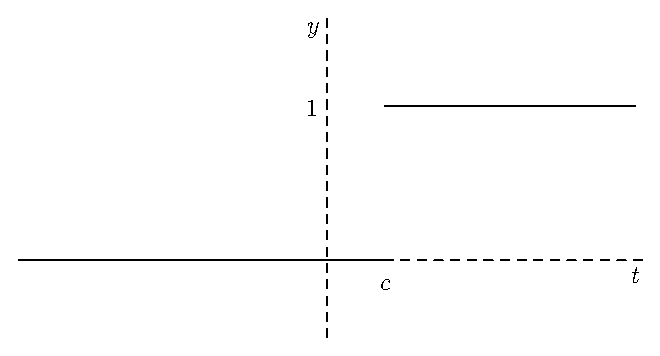
\includegraphics{figures/step}
    \caption{Graph of the step function $u_c(t)$.}
    \label{step}
  \end{center}
\end{figure}

The Laplace transform of the step function is straightforward to calculate. If
we take $c>0$, then
\begin{dmath*}[compact]
  \Laplace{}\(u_c(t)\) 
  = \int_0^\infty u_c(t) e^{-st} dt
  = \int_c^\infty e^{-st} dt
  =\frac{e^{-cs}}{s}.
\end{dmath*}
The step function often shows up multiplied by other functions, but it's easy
to spot. Whenever you have an exponential in the frequency domain, the 
inverse Laplace transform involves a step function: just use the formula
\begin{dmath*}
  \boxed{\Laplace\[u_c(t) f(t-c)\] = e^{-cs} F(s).}
\end{dmath*}

\workedexample{Solve the differential equation
\begin{dmath*}[compact]
  y'=t u_c(t), \qquad y(0)=0
\end{dmath*}
using Laplace transforms.\\
}
{\\\indent
Take the Laplace transform of both sides of the differential equation, yielding
\begin{dmath*}
  sY 
  = \Laplace{}\[t u_c(t)\]
  = \Laplace{}\[ u_c(t) (t-c)\]  + c \Laplace\[u_c(t)\]
  = e^{-cs} \frac{1}{s^2}  + c \frac{e^{-cs}}{s}
\end{dmath*}
Thus,
\begin{dmath*}
  Y 
  = \frac{ce^{-sc}}{s^2} +\frac{e^{-sc}}{s^3}.
\end{dmath*}
From the table of Laplace transforms, we know that
$\Laplace{}\(f(t-c)u_c(t)\)=e^{-cs}F(s)$, so
\begin{dmath*}
  y = c(t-c)u_c(t) + \frac{1}{2} (t-c)^2 u_c(t). 
\end{dmath*}\qed
}



\section{The Impulse Function}
While the step function describes functions which start suddenly (like turning
on a switch), the delta function, $\d(t)$, is slightly more complicated. It
describes processes that happen in an instant, like the impact from a hammer.
It is (loosely) defined as having the following properties:
\be
\boxed{
\delta(t) = \left\{ \begin{array}{ll}
         \infty & \mbox{if $t = 0$};\\
        0 & \mbox{if $t \neq 0$}.\end{array} \right.
}
\ee
and, for any function $f(t)$,
\be \label{deltaprop}
\boxed{\int_{-\infty}^\infty f(t) \delta(t)\, dt = f(0)}.
\ee
% FIXME: this figure isn't very good.
%Approximations to the delta function are shown in figure~\ref{deltafig}.
%\begin{figure}[htbp]
%  \begin{center}
%    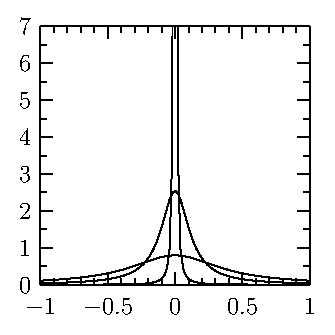
\includegraphics{figures/delta}
%    \caption{Approximations to $\d(x)$.}
%    \label{deltafig}
%  \end{center}
%\end{figure}


\noindent\emph{Example}: Solve the following differential equation using
Laplace transforms.
\begin{dmath*}[compact]
  2y'' + y' + 2y = \delta(t-5), \qquad y'(0)=y(0)=0
\end{dmath*}
\emph{Solution}: Taking the Laplace transform of both sides, we have
\begin{dmath}
  \label{exeq1}
  \(2s^2 + s +2\) Y = e^{-5s}.
\end{dmath}
To see that the Laplace transform of $\delta(t-5)$ is $e^{-5s}$, consider the
definition of the Laplace transform:
\be
\Laplace(\delta(t-5)) = \int_0^{\infty} e^{-st} \delta(t-5)\, dt.
\ee
If we let $\tau = t-5$, then this is the same as
\begin{dmath*}
  \int_{-5}^{\infty} e^{-s(\tau+5)} \delta(\tau)\, d\tau .
\end{dmath*}
Then we apply equation~\eqref{deltaprop} to see that this is just $e^{-5s}$.

Going back to equation~\eqref{exeq1}, solving for $Y$ and completing the
square yields
\begin{dmath*}
  Y = \frac{e^{-5s}}{2} \( \frac{1}{\(s+\frac{1}{4}\)^2 + \frac{15}{16}} \).
\end{dmath*}
Finding the inverse transform is the hardest part of this process, but we can
break it up into smaller steps. We can just pull the $1/2$ out
because the Laplace transform is linear and then if we rearrange this, we get
\begin{dmath*}
  Y = \frac{2}{\sqrt{15}}  \, e^{-5s}
\frac{\sqrt{\frac{15}{16}}}{\(s+\frac{1}{4}\)^2 + \frac{15}{16}}
= \frac{2}{\sqrt{15}}  \, e^{-5s} \,
\Laplace\[e^{\frac{-t}{4}}\sin\(\frac{\sqrt{15}}{4}t \) \]
\end{dmath*}
Now we have an exponential term, $e^{-5s}$, times a term that is the Laplace
transform of $e^{\alpha t}\sin(\beta t)$ with $\alpha=1/4$ and
$\beta=\sqrt{{15}/{16}}$. So we will use the Laplace
transform table to see that $Y$ is the Laplace transform of
\begin{dmath*}
  y
  =\frac{2}{\sqrt{15}}u_5(t) e^{\frac{-(t-5)}{4}}\sin\(\frac{\sqrt{15}}{4}(t-5)\)
  .
\qed
\end{dmath*}

\section{Problems}
\begin{enumerate}
\item Solve the integro-differential equation
  \begin{dmath*}
    y(t) + \int_0^t y(v) (t-v) dv = 1.
  \end{dmath*}
  \hidesolution{
    \begin{dmath*}
    \int_0^t y(v) (t-v) dv = \int_0^t (t-v) y(v) dv = t \ast y(t)
    \end{dmath*}
    so this equation is
    \begin{dmath*}
    y(t) + t \ast y(t) = 1.
    \end{dmath*}
    Recall that
    \begin{dmath*}
    \Laplace \{f \ast g\} = \Laplace \{f\} \Laplace \{g\}
    \end{dmath*}
    so the Laplace transform of this equation is
    \bee
    \Laplace \{y(t)\} + \Laplace \{ t \ast y(t) \} &=& \Laplace \{1 \} \\
    \Laplace \{y(t)\} + \Laplace \{t\} \Laplace \{y(t)\} &=& \Laplace \{1\} \\
    Y(s) + \frac{1}{s^2} Y(s) &=& \frac{1}{s} \\
    \left( 1 + \frac{1}{s^2} \right) Y(s) &=& \frac{1}{s} \\
    \frac{s^2 + 1}{s^2} Y(s) &=& \frac{1}{s} \\
    Y(s) &=& \frac{s^2}{s(s^2+1)} \\
    Y(s) &=& \frac{s}{s^2+1}.
    \eee
    Then taking the inverse transform yields
    \begin{dmath*}
    y(t) = \Laplace^{-1} \( \frac{s}{s^2+1} \) = \cos t.
    \end{dmath*}
  }

  \item
    Find the Laplace transform of
    \begin{dmath*}
    f =
    \left\{ \begin{array}{ll}
      e^t & \mbox{if $t < c$};\\
      t^2 & \mbox{if $t \geq c$}.
    \end{array} \right.
    \end{dmath*}
    \hidesolution{
      \begin{dmath*}
        \Laplace(f)
        = \int_0^c e^t e^{-st} \, dt + \int_c^\infty t^2 e^{-st} \, dt
      \end{dmath*}
      The first integral is
      \begin{dmath*}
        \int_0^c e^t e^{-st} \, dt 
        = \left.\frac{e^{(1-s)t}}{1-s}\right|_0^c
        =\frac{e^{(1-s)c}-1}{1-s}.
      \end{dmath*}
      The second integral requires two integrations-by-parts:
      \begin{dmath*}
        \int_c^\infty t^2 e^{-st} \, dt
        = \left. t^2 \frac{e^{-st}}{-s}\right|_c^\infty
        -2 \int_c^\infty t \frac{e^{-st}}{-s} \, dt
        =\frac{c^2}{s} +\frac{2}{s}
        \[
        t \left.\frac{e^{-st}}{-s}\right|_c^\infty
        - \int_c^\infty \frac{e^{-st}}{-s}\,dt
        \]
        =\frac{c^2}{s} + \frac{2c}{s^2} + \frac{2}{s^3}.
      \end{dmath*}
      The Laplace transform of $f$ is then the sum, i.e.,
      \begin{dmath*}
        \Laplace(f) =
        \frac{e^{(1-s)c}-1}{1-s}
        + \frac{c^2}{s} + \frac{2c}{s^2} + \frac{2}{s^3}.
      \end{dmath*}
    }

\item
  Prove that $\Laplace(f*g)=F(s)G(s)$.
  \hidesolution{TODO: write solution.}

\item
  Solve $y'' = t\times u_c(t)$, $y(0)=y'(0)=0$, for $y(t)$ using Laplace 
  transforms.
  \hidesolution{
    Note that $tu_c(t) = (t-c)u_c(t) +cu_c(t)$. Then,
    \begin{dmath*}
    s^2 Y = \frac{e^{-cs}}{s^2} + \frac{e^{-cs}}{s},
    \implies Y =  \frac{e^{-cs}}{s^4} + \frac{e^{-cs}}{s^3}
    \end{dmath*}
    so
    \begin{dmath*}
    y = u_c(t) \(\frac{t^3}{3!} + \frac{t^2}{2!}\).
    \end{dmath*}
  }

\item
  Solve the IVP
  \begin{dmath*}[compact]
    y'' + y = M\d(t-1), \qquad y'(0)=y(0)=0.
  \end{dmath*}
  \hidesolution{
    Taking the Laplace transform yields $ s^2 Y + Y = M e^{-s}$. Solving for
    $Y$ gives $Y= M e^{-s}\frac{1}{1+s^2}$, which has inverse Laplace 
    transform $y(t) = M u_1(t) \sin(t-1)$.
  }

\end{enumerate}



\chapter{Solving Systems of Differential Equations}
\ifthenelse{\value{small}=1}{\newpage}

Up to now, we could have solved every problem with the method of variation
of parameters. You've probably noticed that some questions are easier to
solve with certain techniques than with others, of course, but VoP will handle
any nonhomogeneous part, so long as you can calculate the integral. Here's
something that it won't handle:
\\

\noindent\emph{Example}:
Solve the system of initial value problems for both $x$ and $y$:
\bee
x' &=& -y \qquad x(0)=0 \\
y' &=& \phantom{-}x \qquad y(0)=1 \\
\eee
Well, you can actually solve this by doing tricky things like taking the
derivative of one of the equations, but let's use Laplace transforms:
\\

\noindent\emph{Solution}: The Laplace transform of the original system is
\bee
sX &=& -Y \\
sY-1 &=&\phantom{-}X.
\eee
Solving for $Y$ yields
\be
\label{syseg1}
sY -1 = \frac{-Y}{s} \quad \implies \quad Y = \frac{s}{s^2+1}.
\ee
Taking the inverse Laplace transform of equation~\eqref{syseg1} gives us
\begin{dmath*}
y(t) = \cos t.
\end{dmath*}
We can solve for $X$ in a similar way, or just notice that $x=y'$, i.e.\
\begin{dmath*}
x(t) = -\sin t.
\end{dmath*}

Systems of differential equations model situations where there are two
or more quantities are changing in time, for example heat and reaction
rate, or predator and prey populations. While they are obviously of
great use, they can get quite complicated as the number of variables
increases (and are greatly simplified by writing them in terms of
matrices).\\


\noindent\emph{Example}: Solve the following system of differential equations:
\bee
x' - 3x + 2y = \sin t\\
4x -y' - y = \cos t
\eee
with initial conditions $x(0)=y(0)=0$.
\\

\noindent\emph{Solution}:\\
We take the Laplace transform of each equation and put in the initial
conditions, which yields
\bee
sX - 3X +2Y = \frac{1}{s^2+1}\\
4X -sY -Y = \frac{s}{s^2+1}.
\eee
We can solve the second equation for X:
\begin{dmath*}
  X = \frac{1}{4}\(\frac{s}{s^2+1} + (s+1)Y\)
\end{dmath*}
Put this into the first equation, so
\begin{dmath*}
\(s-3\)\(\frac{1}{4} \frac{s}{s^2+1} + \frac{s+1}{4}Y\) +2Y
= \frac{1}{s^2+1}
\end{dmath*}
which gives
\begin{dmath}
  \label{sysY}
  Y 
  = -\frac{(s-4)(s+1)}{(s^2+1)(s^2-2s+5)}
  = \frac{11s +7}{10(s^2+1)} + \frac{-11s + 5}{10(s^2-2s+5)}
  = \frac{11s}{10(s^2+1)} + \frac{7}{10(s^2+1)} +
  \frac{-11}{10}\frac{s-1}{(s-1)^2 + 2^2}
  -  \frac{3}{10}\frac2{(s-1)^2 + 2^2}
\end{dmath}
by partial fractions and completing the square in the last two terms. We are
now in a position to use an inverse Laplace transform to get $y(t)$:
\begin{dmath*}
  y(t) = \frac{7}{10} \sin t + \frac{11}{10} \cos t
  - \frac{11}{10}e^{t}\cos 2t - \frac{3}{10}e^{t}\sin 2t
\end{dmath*}
It now remains to solve for $x(t)$. We use the solution for $X$
and the Laplace transform of $y$. This is to say
\begin{dmath}
  \label{sysX}
  X 
  = \frac{1}{4}\(\frac{s}{s^2+1} + (s+1)Y\)
  = \frac{-1 + 7s}{10(s^2+1)} + \frac{-7s + 15}{10(s^2-2s+5)}
 = \frac{7s}{10(s^2+1)} + \frac{-1}{10(s^2+1)} + \frac{-7}{10}
 \frac{s-1} {(s-1)^2 + 2^2} +  \frac{2}{5}\frac{2}{(s-1)^2 + 2^2}
\end{dmath}
So we can now use an inverse Laplace transform to get $x(t)$.
\begin{dmath*}
x(t) = \frac{-1}{10} \sin t + \frac{7}{10} \cos t - \frac{7}{10}e^{t}\cos 2t
+ \frac{2}{5}e^{t}\sin 2t
\end{dmath*}

Alternatively, we could have solved this as a linear system, since
\begin{dmath*}
\[ \begin{array}{ll}
    (s-3) & 2\\
    4 & -(s+1)
  \end{array} \]
\( \begin{array}{l}
    X\\
    Y
  \end{array} \)
=
\( \begin{array}{l}
    \frac{1}{s^2+1}\\
    \frac{s}{s^2+1}
  \end{array} \)
\end{dmath*}
which is easily solved for $X$ and $Y$ to give
\begin{dmath*}
\( \begin{array}{l}
    X\\
    Y
  \end{array} \)
=
\frac{1}{s^2+1} \cdot \frac{1}{s^2-2s+5}
\( \begin{array}{l}
    3s+1\\
    s^2 -3s -4
  \end{array} \),
\end{dmath*}
which brings us to equations~\eqref{sysY} and~\eqref{sysX} with a lot less
work. \qed

\section{Problems}

\begin{enumerate}
  \item Solve the following system of differential equations:
    \begin{dmath*}
      \begin{array}{ll}
        x'=z, & \qquad x(0)=0\\
        y'=x, &\qquad y(0)=0 \\
        z'=y, &\qquad z(0)=1.
      \end{array}
    \end{dmath*}
    \hidesolution{
      Note: For the quiz, computing just $z(t)$ should be sufficient, since this
      takes students about 40 minutes.\\

      The Laplace transform gives us
      \begin{dmath*}[compact]
        sX = Z 
        sY = X 
        sZ-1 = Y
      \end{dmath*}
      Solving for $Z$, we have
      \begin{dmath*}
        Z = \frac{s^2}{s^3-1}
        = \frac{1}{3}\frac{1}{s-1}
        + \frac{1}{3} \frac{2s+1}{s^2 + s+ 1}
        = \frac{1}{3}\frac{1}{s-1}
        + \frac{1}{3} \frac{2s+1}{(s+\half)^2+ \frac{3}{4}}
        = \frac{1}{3}\frac{1}{s-1}
        + \frac{2}{3} \frac{s+\half}{(s+\half)^2+ \frac{3}{4}}
      \end{dmath*}
      which has inverse Laplace transformation
      \begin{dmath*}[compact]
        z = \frac{1}{3}e^t
        + \frac{2}{3}e^{-\frac{t}{2}} \cos \frac{\sqrt{3}}{2} t.
      \end{dmath*}
      Similarly, $sX=Z$ implies that
      \begin{dmath*}
        X = \frac{s}{s^3 -1}
        = \frac{1}{3}\frac{1}{s-1} - \frac{1}{3}\frac{s-1}{s^2+s+1}
        = \frac{1}{3}\frac{1}{s-1}
        - \frac{1}{3}\frac{s+\half}{(s+\half)^2+\frac{3}{4}}
        - \frac{1}{3}\frac{-3}{2}\frac{2}{\sqrt{3}}
        \frac{\sqrt{3}/2}{(s+\half)^2+\frac{3}{4}}
      \end{dmath*}
      so
      \begin{dmath*}
        x = \frac{e^t}{3}
        -e^{\frac{-t}{2}}\(
        \frac{1}{3}\cos \frac{\sqrt{3}}{2}t
        +\frac{1}{\sqrt{3}}\sin \frac{\sqrt{3}}{2}t
        \),
      \end{dmath*}
      and $sY=X$ implies that
      \begin{dmath*}
        Y = \frac{1}{s^3-1}
        = \frac{1}{3}\frac{1}{s-1} - \frac{1}{3}\frac{s+2}{s^2+s+1}
        = \frac{1}{3}\frac{1}{s-1}
        - \frac{1}{3}\frac{s+\half}{(s+\half)^2+\frac{3}{4}}
        - \frac{1}{3}\frac{3}{2}\frac{2}{\sqrt{3}}
        \frac{\sqrt{3}/2}{(s+\half)^2+\frac{3}{4}}
      \end{dmath*}
      so
      \begin{dmath*}
        Y = \frac{e^t}{3}
        +e^{\frac{-t}{2}}
        \(
        \frac{1}{3}\cos \frac{\sqrt{3}}{2}t
        -\frac{1}{\sqrt{3}}\sin \frac{\sqrt{3}}{2}t
        \).
        \qed
      \end{dmath*}
    }

  \item
    Solve the following system of differential equations
    \bee
    x' -y = e^t, \qquad x(0)=1.
    \\
    y' + x = e^t, \qquad y(0)=0.
    \eee
    \hidesolution{
      The transform gives us
      \bee
      sX -1 -Y = \frac{1}{s-1}
      \\
      sY + X = \frac{1}{s-1}
      \eee
      so
      \begin{dmath*}
        s^2 Y  + Y = \frac{-1}{s-1} -1 + \frac{s}{s-1}
        =- \frac{1}{s-1} -1 + \frac{s-1}{s-1} - \frac{1}{s-1}
        = \frac{-2}{s-1}.
      \end{dmath*}
      Thus,
      \begin{dmath*}
        Y = \frac{-2}{3} \(-\frac{s+1}{s^2+1} + \frac{1}{s-1} \)
      \end{dmath*}
      so
      \begin{dmath*}
        y = \frac{2}{3}\sin t + \frac{2}{3}\cos t - \frac{2}{3}e^t
        \text{ and } x = e^t-y'
        = -\frac{2}{3}\cos t + \frac{2}{3} \sin t + \frac{5}{3}e^t
        .\qed
      \end{dmath*}

    }

    \item
      Solve the system of differential equations
      \bee
      x'+y=0,\qquad x(0)=1
      \\
      y' = 2 \cosh(2t),\qquad y(0)=1
      \eee
      \hidesolution{
      The second DE has transform
      \begin{dmath*}
      sY -1 = 6 \frac{s}{s^2-4} \implies Y =  6 \frac{1}{s^2-4} + \frac{1}{s}
      \end{dmath*}
      so
      \begin{dmath*}
      y = \sinh(t) +1
      \end{dmath*}
      and
      \begin{dmath*}
      x = \int \sinh(t) +1 dt = \cosh t +t +C
      \end{dmath*}
      with $C=0$ matching the initial condition. \qed
      }

\end{enumerate}


\chapter{Series Solutions to DEs}
\ifthenelse{\value{small}=1}{\newpage}

An appropriately smooth function $f(t)$ may be represented as a 
\emph{Taylor series},
\begin{dmath*}
  \boxed{f(t)=\sum_{i=0}^\infty \frac{f^{(i)}(a)}{i!}(t-a)^i}.
\end{dmath*}
The Taylor series breaks $f(t)$ up into powers of $t$; this can be
very useful in solving some differential equations.  It's important to when
a series solution is valid, which is to say, when the Taylor series
converges to the value of the function. To answer this question, we have
a variety of tests:
\begin{enumerate}
\item \emph{The comparison test}: if $\lim_{n \rightarrow \infty}
  \abs{a_n/b_n} \in (0,\infty)$, then $\sum_{n=0}^\infty a_n$
  converges if and only if $\sum_{n=0}^\infty b_n$ converges.
\item \emph{The ratio test}: if
  $\lim_{n\rightarrow\infty}\abs{\frac{a_{n+1}}{a_n}}=c < 1$, then
  $\sum_{n=0}^\infty a_n$ converges.
\item \emph{The root test}: if $\lim_{n\rightarrow\infty}\abs{a_n}^{1/n}=c < 1$,
  then $\sum_{n=0}^\infty a_n$ converges.
\item \emph{The integral test}: if there is a function $f$ with
  $f(n)=a_n$, then $\sum_{n=0}^\infty a_n$ converges if and only if
  $\int_0^\infty f(t) dt$ is finite.
\item \emph{The alternating series test}: if $a_n = (-1)^n c_n$, $c_n \geq
  0$, then $\sum_{n=0}^\infty a_n$ converges so long as
  $\lim_{n\rightarrow\infty}c_n=0$ and $c_{n+1} < c_n$ for large
  enough $n$.
\end{enumerate}
If we know the Taylor series, we can use these tests to determine the
range in which the series equals the function. If you try and get a
solution outside of this range, you might get an answer, but it's not
going to be a correct one.
\\

\workedexample{
  Find the Taylor series for $f=e^x$ about $x=0$ and determine its interval of
  convergence.

}{
  First, we need to find the derivatives of $e^x$. This is easy, since
  \begin{dmath*}[compact]
    f^{(n)}(x) = \frac{d^n}{dx^n}e^x = e^x.
  \end{dmath*}
  Thus, $f^{(n)}(0)=e^0=1$, so the Taylor series is given by
  \begin{dmath*}
    \sum_{n=0}^\infty \frac{1}{n!} x^n.
  \end{dmath*}
  For what values of $x$ will this series converge? To determine this, we'll
  have to use a convergence test. Our test are:
  Let's try the ratio test. That is, fix $x$ and look at
  \begin{dmath*}[compact]
    \lim_{n\rightarrow\infty} \frac{a_{n+1}}{a_n}
    = \lim_{n\rightarrow\infty}\frac{x^{n+1}/(n+1)!}{x^n/n!}
    =\lim_{n\rightarrow\infty}\frac{x}{n+1} =0 < 1.
  \end{dmath*}
  That is, for any $x\in \mathbb{R}$, $n+1$ will eventually be greater than
  $x$.  Thus, the limit is zero, and the series converges for all
  $x \in (-\infty,\infty) =\mathbb{R}$. \qed
}

In the above example, the series converged everywhere. This isn't always
the case: often, a series solution to a differential equation is only
valid in some neighbourhood of the initial conditions, and the series
becomes divergent when $\abs{t-a} > r$, and we call $r$ the \emph{radius of
convergence}.

%\workedexample{
%  Find the radius of convergence for the Taylor series for $f=\arctan(x)$
%  about $x=0$.\\
%}
%{
%
%  The Taylor series for $\arctan(z)$ is
%  \begin{dmath*}
%  \sum_{n=0}^\infty \frac{(-1)^n z^{2n+1}}{2n+1}
%  \end{dmath*}
%  Using the ratio test again, we look at
%  \begin{dmath*}
%  \abs{\frac{a_{n+1}}{a_n}} = \frac{z^{2(n+1)+1}/(2(n+1)+1)}{z^{2n+1}/(2n+1)}
%  = \frac{z^2}{(2n+3)/(2n+1)}\rightarrow z^2
%  \end{dmath*}
%  Clearly, this limit is only less than one if $\abs{z}<1$. We still need to
%  check the case when $\abs{z}=1$. This is pretty easy to do, since if $z=1$,
%  the series is just
%  \begin{dmath*}
%  \sum_{n=0}^\infty \frac{(-1)^n}{2n+1},
%  \end{dmath*}
%  which converges by the alternating series test. Similarly, the series
%  converges if $z=-1$. Thus, the interval of convergence is $\[-1,1\]$.
%  \qed
%}

Now that we can calculate Taylor series and know when they are valid,
we can use them to calculate solutions to differential equations. To
simplify matters, we will restrict ourselves to initial value problems
which begin at $t=0$, so that $a=0$ in all the above formulae. Now, we
can express the solution $y(t)$ as a power series,
\begin{dmath}
  \label{pseries}
  y(t) = \sum_{n=0}^\infty a_n t^n .
\end{dmath}
which is really just a Taylor series:
\begin{dmath}
  \label{tseries}
  y(t) = \sum_{n=0}^\infty \frac{y^{(n)}(0)}{n!} t^n .
\end{dmath}
Since Taylor series are unique, equations~\eqref{pseries}
and~\eqref{tseries} must agree term-by-term.  That is, for
$n=0,1,2,\dots$,
\begin{dmath*}
  a_n = \frac{y^{(n)}(0)}{n!}.
\end{dmath*}
That is, initial conditions specify coefficients: if you are given
$y(0)=c_0$, then you know that 
\begin{dmath*}
  a_0 = y(0)/0! = c_0.
\end{dmath*}
 Similarly, $y'(0)=c_1$ specifies $a_1$, and so on.

We assume that this solution is analytic, so we can take the
derivative of the series term-by-term. That is,
\begin{dmath*}[compact]
  \dd{y}{t} 
  = \dd{}{t}\sum_{n=0}^\infty a_n t^n
  = \sum_{n=0}^\infty \dd{}{t}\(a_n t^n\)
  = \sum_{n=0}^\infty a_n n t^{n-1}
  = \sum_{n=1}^\infty a_n n t^{n-1}.
\end{dmath*}
The last equality is because when $n=0$ we have that $a_0 \times
0\times t^{0-1}=0$, so we can ignore this term.

To solve differential equations using power series, we put the power
series representation for $y(t)$, $y'(t)$, and so on, into the
differential equation.  Matching like powers of $t$ gives us a a
recurrence relation, which expresses $a_n$ in terms of $a_m$ with $m <
n$, which we can solve to get $a_n$ in terms of $n$ and the initial
conditions.
\\

%\workedexample{Determine the solution to the IVP
%\begin{dmath*}[compact]
%  y'(t) = t^2 +t, \qquad y(0)=1
%\end{dmath*}
%using a Taylor series for $y$.\\
%}
%{
%  Let $y =\sum_{n=0}^\infty a_n t^n$.  Then, $a_0=y(0)=1$, and
%  \begin{dmath*}
%    y'(t) = \sum_{n=1}^\infty a_n n  t^{n-1} = t^2 +t.
%  \end{dmath*}
%  Matching like powers of $t$, we have
%  \begin{dmath*}[compact]
%    2 a_2 t = t, \qquad 3 a_3 t^2 = t^2
%  \end{dmath*}
%  and $a_n n t^n =0$ for $n=1$ and all $n \geq 4$. Thus, $a_1 =0$, $a_2=\half$,
%  and $a_3 = \frac{1}{3}$. The solution is then
%  \begin{dmath*}
%    y(t) = 1 +\frac{t^2}{2} +\frac{t^3}{3}.
%  \end{dmath*}
%}
%It was easy to isolate all of the $a_n$'s in the previous example, since $y'$
%appeared alone in the IVP. It's usually necessary to solve for $a_n$
%recursively.\\
\workedexample{
  Solve the IVP
  \begin{dmath*}[compact]
  y'' = -y, \qquad y(0) =1, \qquad y'(0)=0.
  \end{dmath*}
  using a Taylor series for $y$.\\
}
{

  Again, let $y=\sum_{n=0}^\infty a_n t^n$. Then
  \begin{dmath*}
    y'' = \sum_{n=2}^\infty a_n n (n-1)t^{n-2}.
  \end{dmath*}
  The differential equation is then
  \begin{dmath}
    \label{serieseg}
    \sum_{n=2}^\infty a_n n (n-1)t^{n-2} = -\sum_{n=0}^\infty a_n t^n
  \end{dmath}
  If we set $m=n-2$, then we can shift the summation index on the LHS to start
  at zero. That is,
  \begin{dmath*}
    y'' = \sum_{n=2}^\infty a_n n (n-1)t^{n-2}
    = \sum_{m=0}^\infty a_{m+2}(m+2)(m+1)t^m.
  \end{dmath*}
  This makes it much easier to solve equation~\eqref{serieseg}, since
  we now have
  \begin{dmath*}[compact]
    \sum_{m=0}^\infty a_{m+2}(m+2)(m+1)t^m =  -\sum_{n=0}^\infty a_n t^n
  \end{dmath*}
  and we can put it all together to get
  \begin{dmath*}
    \sum_{n=0}^\infty \[a_{n+2}(n+2)(n+1) +a_n \]t^n =0
  \end{dmath*}
  In order for this to hold for all $t$ in a neighbourhood of $t=0$, it must
  be that
  \begin{dmath*}
    a_{n+2}(n+2)(n+1) +a_n =0
  \end{dmath*}
  which gives us the recurrence relation
  \begin{dmath}
    \label{seriesrec}
    a_{n+2}= \frac{-a_n}{(n+2)(n+1)}.
  \end{dmath}
  From the initial conditions, we have $a_0=1$ and $a_1=0$. We can
  solve for $a_2$ by setting $n=0$ in equation~\eqref{seriesrec},
  which yields $a_2=-\half$.

  If we have $n$ even, then $n=2p$, and
  \begin{dmath*}
    a_{2p} 
    = -\frac{a_{2p-2}}{2p(2p-1)} 
    = \frac{a_{2p-4}}{2p(2p-1)(2p-3)(2p-4)}
    = \frac{(-1)^p a_0}{(2p)!} =\frac{(-1)^p}{(2p)!}
  \end{dmath*}
  It's easy to see that $a_3=0$, and, in fact, $a_n=0$ if $n$ is odd. Since
  we now know the values for all the $a_n$, we can write the solution:
  \begin{dmath*}
    y(t) = \sum_{n=0}^\infty t^n
    \left\{\begin{array}{ll}
    \frac{(-1)^{n/2}}{n!} & \mbox{if $n$ is even};\\
    0 & \mbox{if $n$ is odd}.
    \end{array} \right.
    = \sum_{p=0}^\infty \frac{(-1)^p t^{2p}}{(2p)!}. 
  \end{dmath*}
 You may recall from previous classes that this is just the Taylor series
 for $\cos t$. \qed
}

Sometimes we just don't know how to solve a differential equation, and
the best that we can do is to give an approximation of the solution
which is valid over some range. One way to do this is to use the
\emph{Taylor Polynomial Approximation} (or simply a Taylor
polynomial). It's easy to deal with both analytically and numerically,
and it can be used to get at least a basic understanding of just about
any initial value problem. The $n$th degree Taylor polynomial is
\begin{dmath*}
%FIXME: the boxed command doesn't wrap lines, so it's removed for the ebook
%  \boxed{
    f_n(t) 
    = f(a) + f'(a)(t-a) + \dots + \frac{f^{(n)}(a)}{n!} (t-a)^n
    = \sum_{i=0}^n \frac{f^{(i)}(a)}{i!}(t-a)^i
%  }
,
\end{dmath*}
and it exists for any function $f$ whose first $n$ derivatives are
smooth for $t\in [a,t]$.  Let $R_n(t) = f(t) -f_n(t)$ denote the error
associated with the $n$th Taylor polynomial. Then, Taylor's theorem
states that there exists a number $\xi \in [a,t]$ where
\begin{dmath*}
  \boxed{R_n(t) = \frac{f^{(n+1)}(\xi)}{(n+1)!}(t-a)^{n+1}}.
\end{dmath*}
So long as $\lim_{n\rightarrow \infty} R_n(t) =0$, $f_n$ will be a better and
better approximation as $n$ increases.

%FIXME: put an example where we just find a couple of terms?

\section{Problems}
\begin{enumerate}
\item Determine the convergence set of the series
  \begin{dmath*}
    \sum_{n=0}^\infty \frac{3^n}{n} (x-2)^n.
  \end{dmath*}
  \hidesolution{
    For this series $a_n = \frac{3^n}{n}$ and $x_0 = 2$, so
    \begin{dmath*}
      L 
      = \lim_{n \to \infty} \left| \frac{a_{n+1}}{a_n} \right|
      = \lim_{n \to \infty} \left| \frac{3^{n+1}}{n+1} / \frac{3^n}{n} \right|
      = \lim_{n \to \infty}
      \left| \frac{3 \cdot 3^n}{n+1} \times \frac{n}{3^n} \right|
      = \lim_{n \to \infty} \left| 3 \frac{n}{n+1} \right|
      = 3 \lim_{n \to \infty} \frac{n}{n+1}
      = 3
    \end{dmath*}
    and then $\rho = \frac{1}{L} = \frac{1}{3}$. So the series converges 
    (absolutely) on
    \begin{dmath*}
    (x_0 - \rho, x_0 + \rho) = \left( 2 - \frac{1}{3}, 2 + \frac{1}{3} \right)
    = \left( \frac{5}{3}, \frac{7}{3} \right).
    \end{dmath*}
    It remains to check if the series converges at the endpoints of this
    interval.  At $x = \frac{5}{3}$, we have
    \begin{dmath*}[compact]
      \sum_{n=0}^\infty \frac{3^n}{n} \left( \frac{5}{3} - 2 \right)^n
      = \sum_{n=0}^\infty \frac{3^n}{n} \left( \frac{-1}{3} \right)^n
      = \sum_{n=0}^\infty \frac{3^n}{n} \times \frac{(-1)^n}{3^n}
      = \sum_{n=0}^\infty \frac{(-1)^n}{n}
    \end{dmath*}
    which is the alternating harmonic series which converges (recall that an
    alternating series converges $\iff$ the terms go to 0),
    and at $x = \frac{7}{3}$ we have
    \begin{dmath*}[compact]
      \sum_{n=0}^\infty \frac{3^n}{n} \left( \frac{7}{3} - 2 \right)^n
      = \sum_{n=0}^\infty \frac{3^n}{n} \left( \frac{1}{3} \right)^n
      = \sum_{n=0}^\infty \frac{1}{n}
    \end{dmath*}
    which is the harmonic series which diverges. So the convergence set is
    $\left[ \frac{5}{3}, \frac{7}{3} \right)$.
  }

  \item
    Determine the first four non-zero terms of the Taylor series of the
    solution to the Chebyshev equation,
    \begin{dmath*}
      (1-x^2)y'' - xy' +p^2 y=0
    \end{dmath*}
    with initial conditions $y(0)=a_0$, $y'(0)=a_1$.
    \hidesolution{
      TODO: write the solution
    }

%  \item
%    Determine the fourth degree Taylor polynomial for the solution to
%    \begin{dmath*}[compact]
%    (y')^2 + y = e^x, \qquad y(0)=0.
%    \end{dmath*}
%    \hidesolution{
%      The first four terms of $y'$ are $a_1 + 2 a_2 x +3 a_3 x^2 + 4 a_4 x^3$.
%      The first four terms of $(y')^2$ are therefore
%      \begin{dmath*}
%        (y') + y \approx a_0+a_1^2 + x\(a_1 +4 a_1 a_2 \)
%        + x^2 \(a_2+ 4a_2^2+6 a_1 a_3 \)
%        +x^3\(a_3 + 8a_1 a_4 +12 a_2 a_3 \)
%      \end{dmath*}
%      and equal
%      \begin{dmath*}
%        e^x \approx 1 + x + \frac{x^2}{2} + \frac{x^3}{6}
%      \end{dmath*}
%      Matching order-by-order, we have
%      \begin{dmath*}
%      \begin{array}{ll}
%	\O(1): & a_0 + a_1^2 =1 \\
%	\O(x): & a_1(1+ 4 a_2) =1\\
%	\O(x^2): & a_2 + 4a_2^2 + 6 a_1 a_3 =\half \\
%	\O(x^3): & a_3 + 8 a_1 a_4 + 12 a_2 a_3=\frac{1}{6} \\
%      \end{array}
%      \end{dmath*}
%      Subbing back into these equations, we get
%      \begin{dmath*}[compact]
%        a_1=1, \qquad a_2 =0, \qquad a_3=\frac{1}{12}, \qquad a_4=\frac{1}{96},
%      \end{dmath*}
%      and
%      \begin{dmath*}
%        y(x) \approx x + \frac{x^3}{12} + \frac{x^4}{96}.
%      \end{dmath*}
%    }
    
  \item
    Solve
    \begin{dmath*}[compact]
      y' = \frac{1}{1+x^2}, \qquad y(0)=0
    \end{dmath*}
    using a Taylor series. Do not leave your solution as an infinite series,
    but equate it to a known function.
    \hidesolution{
      This is just $y(x)=\arctan x$.
    }

%too complicated--needs help
% \item
%    The pendulum is often approximated as a harmonic oscillator. The full
%    system is nonlinear in $y$, since
%    \be
%    y''=-\sin y,
%    \ee
%    which reduces to the usual case, $y''=-y$, for small $y$. A slightly
%    better approximation would be to approximate $\sin$ to higher order, as in
%    \be
%    \label{pend3}
%    y''=-y + \frac{y^3}{3!}.
%    \ee
%    Provide a third-order Taylor polynomial approximation to the solution of
%    \eqref{pend3}.
%
%    If we take \eqref{pend3} and multiply it by $y'$, we can get the energy
%    equation for the system, namely
%    \be
%    y' y'' = \ddt{y'^2/2}
%    = \ddt{}\int^{y(t)}\(-\hat{y} + \frac{\hat{y}^3}{3!}\) d\hat{y}.
%    \ee
%    Thus, the energy of the system, $E=\frac{y'^2}{2}
%    + \int^{y(t)}\(\hat{y} - \frac{\hat{y}^3}{3!}\) d\hat{y}$, is conserved,
%    since
%    \be
%    \ddt{}\(\frac{y'^2}{2}
%    + \int^{y(t)}\(\hat{y} - \frac{\hat{y}^3}{3!}\) d\hat{y}\) =0.
%    \ee
%    Based on the conservation of energy, what do you expect to happen at large
%    $y$? Why might $y''=-y$ be a better approximation at large $y$ than
%    $y''=-y + {y^3}/{3!}$ is?
%    \hidesolution{
%      TODO: work out the approximation
%
%      The reason that the third-order approximation breaks down is that
%      the energy goes to $-\infty$ for large $\abs{y}$, so the solution will
%      grow unboundedly.
%    }

  \item
    Give a recursion formula for $a_n$ if
    \begin{dmath*}
      a_{3n+1} 
      = \frac{a_1}{(3n+1)\times (3n) \times (3n-2) \dots
        6 \times 4 \times \times 3}.
    \end{dmath*}

  \item
    Given the recursion relationship
    \begin{dmath*}
      a_n = \frac{-2}{n^2}a_{n-1},
    \end{dmath*}
    find $a_n$ explicitly.

  \item
    Given the recursion relationship
    \begin{dmath*}
      a_{n+4} = \frac{-k^2}{(n+4)(n+3)} a_{n-1},
    \end{dmath*}
    with $k$ a constant, find $a_n$ explicitly.

  \item Solve the differential equation
    \begin{dmath*}
      y'' - 2 x y' + \l y=0,
    \end{dmath*}
    with $\l$ a constant, using a Taylor series about $x=0$. For what values
    of $\l$ is the solution a polynomial?
%FIXME: does this question need initial conditions to make sense?
    \hidesolution{
      Putting the Taylor series in we get
      \begin{dmath*}
        \sum_{n=2}^\infty a_n n (n-1) x^{n-2} 
        - 2x \sum_{n=1}^\infty a_n n x^{n-1}
        + \l \sum_{n=0}^\infty a_n x^ n=0
      \end{dmath*}
      which gives
      \begin{dmath*}
        \sum_{m=0}^\infty a_{m+2} (m+2)(m+1) t^m
        - 2 \sum_{n=1}^\infty a_n n t^n
        + \l \sum_{n=0}^\infty a_n t^ n=0
      \end{dmath*}
      so, for $n > 0$, $a_{n+2} (n+2)(n+1) - 2 n a_n  + \l a_n =0$.
      The recurrence relation is 
      \begin{dmath*}[compact]
        a_{n+2} = a_n \frac{\l - 2n}{(n+2)(n+1)}, \qquad n > 0.
      \end{dmath*}
      FIXME: is this question right?
    }

  \item 
    Find the general solution to $y''' + \l y =0$.
    \hidesolution{
      Putting the Taylor series in gives
      \begin{dmath*}
        \sum_{n=3}^\infty a_n(n)(n-1)(n-2) t^{n-3} 
        + \l \sum_{n=0}^\infty a_n t^n=0.
      \end{dmath*}
      let $m=n-3$, so
      \begin{dmath*}
        \sum_{m=0}^\infty a_{m+3}(m+3)(m+2)(m+1) t^m
        + \l \sum_{n=0}^\infty a_n t^n=0.
      \end{dmath*}
      The recurrence relation is then 
      \begin{dmath*}
        a_{n+3} = \frac{-\l a_n}{(n+3)(n+2)(n+1)}.
      \end{dmath*}
      This is solved by
      $a_{3n} = -1^n a_0 / (3n)!$, $a_{3n+1} = -1^n a_1 / (3n+1)!$, 
      $a_{3n+2} = -1^n a_2 / (3n+2)!$, so
      \begin{dmath*}
        y(t) = a_0 \sum_{n=0}^\infty \frac{-1^n}{(3n)!}t^{3n}
        +a_1 \sum_{n=0}^\infty \frac{-1^n}{(3n+1)!}t^{3n+1}
        +a_2 \sum_{n=0}^\infty \frac{-1^n}{(3n+2)!}t^{3n+2}.
      \end{dmath*}
    }
  \item
    Find the general solution to $y' = 2xy$.
    \hidesolution{
      The solution is $y=a_0e^{x^2}$.
    }
    
\end{enumerate}



\chapter{Series Solutions to DEs at Regular Singular Points}
\ifthenelse{\value{small}=1}{\newpage}

%Let $p(t), q(t)$ be analytic functions (ie, they admit power series
%representations).
Differential equations of the form
\begin{dmath}
  \label{singode}
  y'' + p(t)y' + q(t)y=0
\end{dmath}
can behave poorly at $t=0$, and may not admit solutions of the form
$y(t) =\sum_{n=0}^\infty a_n t^n$. However, we can still solve these
problem by modifying the series expansion. The easiest case is when
the singular point is a regular singular point, for which we use
\emph{the method of Froebenius}.

\begin{definition}\emph{Singular points.}
  The point $t=0$ is a \emph{singular point} if either $\lim_{t
    \rightarrow 0}p(t)=\infty$ or $\lim_{t \rightarrow 0}q(t)=\infty$.
\end{definition}

\begin{definition}\emph{Regular singular points.}
  The point $t=0$ is a \emph{regular singular point} of
  equation~\eqref{singode} if the two limits $\lim_{t\rightarrow 0} t p(t)
  =p_0$ and $\lim_{t\rightarrow 0} t^2 q(t) =q_0$ exist and are
  finite.
\end{definition}

Series solutions at regular singular points have one solution of the form
\begin{dmath*}
  \boxed{y_1(t) = \sum_{n=0}^\infty a_n t^{n+r}},
\end{dmath*}
for some $r\in\mathbb{C}$ such that $a_0 \neq 0$.

Since we now have one more variable for which to solve (i.e.\ $r$ in addition
to $a_0, a_1,\dots$), we require one more equation in order to determine the
solution uniquely. Then if we take the first and second derivative of
$y(t) = \sum_{n=0}^\infty a_n t^{n+r}$ and put them into the left-hand side of
equation~\eqref{singode}, we can see that the
leading-order (which is to say the $t^{r-2}$) coefficient is
\begin{dmath*}
  a_0 r(r-1)t^{r-2} + a_0 \frac{p_0}{t} r t^{r-1} + a_0 \frac{q_0}{t^2} t^r
\end{dmath*}
In order to satisfy equation~\eqref{singode}, this equation must equal $0$.
We can multiply by $t^2$ and since $a_0 \neq 0$, we see that
\begin{dmath*}
  \boxed{r(r-1) + p_0 r  + q_0=0.}
\end{dmath*}
This is called the \emph{indicial equation}. It's a quadratic so it has two
solutions, $r=r_1,r_2$.

Second-order differential equations always have two independent
solutions.  For regular singular points, there are three cases which
determine the form of $y_2$:
\begin{enumerate}
  \item{If $r_1\neq r_2$, and $r_1-r_2$ is \emph{not} an integer}: \\
    then $\displaystyle y_2=\sum_{n=0}^\infty b_n t^{n+r_2}$.
  \item{If $r_1 = r_2$}: \\
    then $\displaystyle y_2 = \ln(t) y_1(t) + \sum_{n=0}^\infty b_n t^{n+r_1}$.
  \item{If $r_1\neq r_2$, and $r_1-r_2$ \emph{is} an integer}: \\
    then $\displaystyle y_2=C\ln(t) y_1(t) + \sum_{n=0}^\infty b_n t^{n+r_2}$,
    for some $C\in\mathbb{C}$.
\end{enumerate}
Once one has determined $r_1$ and $r_2$, the constants $a_n$ and $b_n$ can
be determined by matching powers as per the previous section.  We're often
only interested in determining $y_1$.
\\

\workedexample{ Consider Bessel's equation,
  \begin{dmath}
    \label{bessel}
    t^2 y'' + ty' + (t^2-\alpha^2)y=0.
  \end{dmath}
}{

  We can divide Bessel's equation by $t^2$ to get it in the form of
  equation~\eqref{singode}, that is
  \begin{dmath*}
    y''  + \frac{1}{t}y' + \(1-\frac{\alpha^2}{t^2}\)y=0,
  \end{dmath*}
  which is clearly singular. We can identify $p=1/t$, and
  $q=1-\frac{\alpha^2}{t^2}$. Then,
  \begin{dmath*}[compact]
    p_0 = \lim_{t\rightarrow 0} t p(t) =1, \quad \text{and}\quad
    q_0 = \lim_{t\rightarrow 0} t^2 q(t) =-\alpha^2.
  \end{dmath*}
  The indicial equation is then
  $r(r-1) +r -\alpha^2 =0 \implies r_{1,2} = \pm \alpha$.  Thus,
  \bee
  y_1\phantom{''} &=& \sum_{n=0}^\infty a_n t^{n+\alpha} \\
  y_1'\phantom{'}  &=& \sum_{n=0}^\infty a_n (n+\alpha)t^{n+\alpha-1}, \\
  y_1'' &=& \sum_{n=0}^\infty a_n (n+\alpha)(n+\alpha-1)t^{n+\alpha-2}.
  \eee
  Putting this into equation~\eqref{bessel}, we have
  \begin{dmath*}
    \sum_{n=0}^\infty a_n\[(n+\a)(n+\a-1) + (n+\a) - \a^2  \]t^{n+\alpha}
    + \sum_{n=0}^\infty a_n t^{n+2+\alpha}=0.
  \end{dmath*}
  Changing the index of the second sum, we have
  \begin{dmath*}
    \sum_{n=0}^\infty a_n\[(n+\a)(n+\a-1) + (n+\a) - \a^2  \]t^{n+\alpha}
    + \sum_{n=2}^\infty a_{n-2} t^{n+\alpha}=0.
  \end{dmath*}
  The $a_0$ and $a_1$ terms are determined by initial conditions. For
  $n\geq 2$, the terms must cancel, so we have
  \begin{dmath*}
    a_n\[\(n+\a\)^2 - \a^2\]t^{n+\alpha}  + a_{n-2} t^{n+\alpha}=0
  \end{dmath*}
  which implies that
  \begin{dmath*}
    a_n = \frac{-a_{n-2}}{\(n+\a\)^2 - \a^2} =  \frac{-a_{n-2}}{n(n+ 2\a)}.
  \end{dmath*}
  Associating $y_1$ with $a_0=1$ and $a_1=0$, we can set $n=2m$, so the
  recursion relationship is
  \begin{dmath*}
    a_{2m} = \frac{-a_{2(m-1)}}{2m (2m+2\a)} = \frac{-a_{2(m-1)}}{2^2m (m+\a)}.
  \end{dmath*}
  Solving the recursion relationship then yields
  \begin{dmath*}
    a_{2m} = \frac{(-1)^ma_0}{2^{2m}m! (m+\a)(m+\a-1)\dots(1+\a)}.
  \end{dmath*}
  The solution is then
  \begin{dmath}
    \label{bessel1}
    y_1 = \sum_{m=0}^\infty
    \frac{(-1)^m}{2^{2m}m! (m+\a)(m+\a-1)\dots(1+\a)(\a)} t^{m+\alpha}.  \qed
  \end{dmath}
  We can simplify this a little by setting $a_0=1/(2^\a\G(\a+1))$. Then we would
  get the standard form of Bessel's function of the first kind of order $\a$,
  \begin{dmath*}
    J_\alpha(t) = \sum_{n=0}^\infty \frac{(-1)^n}{n!\G(1-\a+n)}
    \(\frac{t}{2}\)^{2n-\a}.
  \end{dmath*}
  Here $\G(x)$ is called the Gamma function and it is an extension of the
  factorial function. So in particular, when $\alpha=0$, we get
  \begin{dmath*}
    J_0(t) = \sum_{n=0}^\infty \frac{(-1)^n t^{2n}}{2^{2n}(n!)^2}.
  \end{dmath*}
% Too messy and complicated- fixed above
%  Now, we can simplify this slightly, by using the gamma function. The
%  Gamma function,
%  \be
%  \G(x) = \int_0^\infty t^{x-1} e^{-t} \, dt,
%  \ee
%  is a generalization of the factorial. The key step is that
%  \be
%  \G(x+1) = x \G(x),
%  \ee
%  which can be derived using integration by parts. If $x$ is an integer, this
%  gives us $\G(x+1)=x!$, since $\G(0)=1$. If we set $x=m+\a+1$, then
%  \be
%  \G(m+\a+1) &=& (m+\a) \G(m+\a) = (m+\a)(m+\a-1)\G(m+\a-1) = \dots \\\nonumber
%  &=& (m+\a)(m+\a-1) \dots (2+\a)(1+\a)\G(\a+1).
%  \ee
%  We can then write \eqref{bessel1} as
%  \be
%  y_1 = \sum_{m=0}^\infty
%  \frac{(-1)^m}{2^{2m}m! \G(m+\a+1)/\G(\a+1)} t^{m+\alpha}.
%  \ee
%
%  Setting $a_0=1/(2^\a\G(\a+1))$, we have the standard form of Bessel's
%  function
%  of the first kind of order $\a$,
%  \be
%  J_\alpha(t) = \sum_{n=0}^\infty \frac{(-1)^n}{n!\G(1-\a+n)}
%  \(\frac{t}{2}\)^{2n-\a}. \qed
%  \ee
}



\section{Problems}

\begin{enumerate}

  \item Find a general solution to the Cauchy-Euler (equidimensional) equation,
    \begin{dmath*}
      (\pi x)^2 y'' (x) + \pi(\pi-2)xy' (x) + y(x) = 0
    \end{dmath*}
    for $x>0$.
    \hidesolution{
      Rewrite this equation as
      \begin{dmath*}
        \pi^2 x^2 y'' (x) + (\pi^2 - 2\pi)xy' (x) + y(x) = 0.
      \end{dmath*}
      We substitute $y = x^r$ to find a solution. The indicial equation is
      \begin{dmath*}
        \pi^2 r^2 + (\pi^2 - 2\pi - \pi^2) r + 1 
        = \pi^2 r^2 - 2 \pi r + 1
        = (\pi r - 1)^2 = 0
      \end{dmath*}
      which has repeated root $r = \frac{1}{\pi}$.  So a general solution is
      \begin{dmath*}
        y(x) 
        = C_1 x^{\frac{1}{\pi}} + C_2 x^{\frac{1}{\pi}} \ln x
        = C_1 \sqrt[\pi]{x} + C_2 \sqrt[\pi]{x} \ln x, \quad x \no > 0.
      \end{dmath*}
      % FIXME: check this.
    }

  \item Find the solution to Bessel's equation corresponding to $r=-\a$,
    assuming that $2\a$ is not an integer.
    \hidesolution{
      TODO: add solution
    }

  \item Find the first solution (i.e.\ $y_1$ in the above notation) to the
    differential equation
    \begin{dmath*}
      x^2 y'' - xy' + (1-x)y=0.
    \end{dmath*}
    \hidesolution{
      We have $p=-1/x$ and $q=(1-x)/x^2 = 1/x^2-1/x$. Then
      \begin{dmath*}[compact]
        p_0 = \lim_{x\rightarrow 0^+} x p(x)=-1, \qquad
        q_0 = \lim_{x\rightarrow 0^+} x^2 q(x)=1.
      \end{dmath*}
      The indicial equation is $r(r-1)-r+1=0$ which gives the double
      root $r_1=r_2=1$. Thus, $y_1$ is given by 
      $y = x^1 \sum_{n=0}^\infty a_n x^n$, which gives
      \begin{dmath*}
        \sum_{n=1}a_n(n+1)(n)x^{n+1} - \sum_{n=1}a_n(n+1)x^{n+1}
        + \sum_{n=0}a_nx^{n+1} - \sum_{n=0}a_nx^{n+2}.
      \end{dmath*}
      The order $x$ term cancels out, leaving us free to determine $a_0$ by
      the initial conditions. We are then left with
      \begin{dmath*}[compact]
        \sum_{n=1}^\infty \[a_n(n+1)(n)-a_n(n+1)+a_n - a_{n-1}\]x^{n+1}=0,
      \end{dmath*}
      so  $a_n n^2 = a_{n-1}$, which yields
      \begin{dmath*}
        y_1 = a_0\sum_{n=0}^\infty \frac{x^{n+1}}{(n!)^2}.
      \end{dmath*}
    }

\end{enumerate}



\chapter{Partial Differential Equations}
\ifthenelse{\value{small}=1}{\newpage}

Let $u(x,t)$ be the temperature of a one-dimensional rod with thermal
conductivity $k$. The equation that describes the evolution of $y$ is
called the heat equation:
\begin{dmath*}
  \boxed{  \pp{u}{t} =  k\pptwo{u}{x}. }
\end{dmath*}
This is an important example of a partial differential equation (PDE),
in which the derivatives with respect to one variable are related to
derivatives with respect to another variable, in this case
$\partial/\partial t$ and $\partial/\partial x$.

The basic technique for solving partial differential equations is to
transform it into many ordinary differential equations, which we can then
solve using any of the techniques that we have discussed so far. One
very powerful technique to do this is to transform the function $y$
into a \emph{Fourier series}.

\section{Separation of Variables}
As in the previous section, we use a series solution for $y$ and
expand around $x=0$. However, instead of the coefficients being
constant, we allow them to be functions of time, and, instead of using
$x^n$, we let $X_n(x)$ be a more general function of $x$. That is, we
let
\begin{dmath*}
  \boxed{u(x,t) = \sum_{n=0}^\infty T_n(t) X_n(x).}
\end{dmath*}
As you will see in the next lab, we can choose the functions $X_n$ in
a way that makes the PDE solvable. For now, let's consider the case
where the $X_n$ are either sine or cosine, i.e.\ when $u$ is a Fourier
sine or cosine series.

\section{Fourier Cosine and Sine Series}
Consider functions that are periodic with period $2T$.  If we set $X_n
=\cos(n \pi x/T)$, we have the \emph{Fourier cosine series} for
$f(x)$,
\begin{dmath*}
  \boxed{\frac{a_0}{2} + \sum_{n=1}^\infty a_n \cos\(\frac{n \pi x}{T}\)}
\end{dmath*}
(note the annoying $1/2$ on the first term). Setting $X_n=\sin(n \pi x/T)$,
we get the \emph{Fourier sine series} for $f(x)$,
\begin{dmath*}
  \boxed{\sum_{n=1}^\infty b_n \sin\(\frac{n \pi x}{T}\).}
\end{dmath*}
The coefficients $a_n$ and $b_n$ are determined by integration, with
\begin{dmath}
  \label{fouriercoeff}
  \boxed{a_n = \frac{1}{T} \int_{-T}^T f(x) \cos\(\frac{n \pi x}{T}\) \, dx},
\end{dmath}
and
\begin{dmath*}
  \boxed{b_n = \frac{1}{T} \int_{-T}^T f(x) \sin\(\frac{n \pi x}{T}\) \, dx}.
\end{dmath*}
More generally, the \emph{Fourier series} for $f(x)$ is the sum of these, i.e.\
\begin{dmath*}
  \boxed{\frac{a_0}{2} + \sum_{n=1}^\infty \[ a_n \cos\(\frac{n \pi x}{T}\)
    + b_n \sin\(\frac{n \pi x}{T}\) \]}.
\end{dmath*}
Often, we just look at functions that have period $2\pi$, which makes for the
simpler formulae,
\begin{dmath}
  \label{nicefourier}
  \frac{a_0}{2} + \sum_{n=1}^{\infty} \[ a_n \cos\(nx\)
  + b_n \sin\(nx\) \],\\
  \no{a_n =  \frac{1}{\pi} \int_{-\pi}^{\pi} f(x) \cos\(n x\) \, dx,}\\
  \no{b_n =\frac{1}{\pi} \int_{-\pi}^{\pi} f(x) \sin\(n x\) \, dx,}
\end{dmath}
which we will refer to as ``the'' Fourier series, unless otherwise stated.


Well, now we have yet another series that we can derive from a given function,
but we have to show that the series converges to the function if we
want to do anything useful. For this we have the following lemma:
\begin{theorem}[Riemann-Lebesque lemma]
If $\int_{-\infty}^\infty \abs{f(x)} dx$ exists, then
\begin{dmath*}
  \lim_{z\rightarrow \pm \infty}\int_{-\infty}^\infty f(x) e^{izx} dx =0
\end{dmath*}
which implies that $\lim_{n\rightarrow \infty} a_n =0$ and $
\lim_{n\rightarrow \infty} b_n =0$, and
\begin{dmath*}
  \boxed{
    f(x) = \frac{a_0}{2} + \sum_{n=1}^\infty \[ a_n \cos(nx) + b_n \sin(nx) \].
  }
\end{dmath*}
%FIXME: should the limits of integration be $(-\pi,\pi)$ for the series (as
%opposed to the transform)? Also, uniqueness?
\end{theorem}

The Fourier series is the expression of a function as the sum an
infinite series of waves with different amplitudes. That is, we
transform from ``$x$-space'' to ``frequency-space'', which can be
incredibly useful. For example, the \texttt{Ogg Vorbis} audio format
is just a modified cosine-series. Fourier series (and Fourier
transforms, which are not covered in this course) lie at the heart of
signal analysis. In terms of solving PDEs, we make use of the fact
that
\begin{dmath*}
  \ddtwo{}{x}\sin(\l x) = -\l^2 \sin(\l x),
\end{dmath*}
(i.e.\ that sine is an Eigenfunction of $d^2/dx^2$) to turn
differential equations into algebraic equations. But more on that
later. First, let's just find the Fourier series for a normal
function.

\workedexample{
  Find the Fourier series of $f(x) = x$ for $x\in(-\pi,\pi)$.\\
}{\\\indent
  To find the Fourier series, we just need to determine $a_n$ and $b_n$ using
  equation~\eqref{nicefourier}. The coefficients for the cosine series are
  \begin{dmath*}
    a_n 
    = \frac{1}{\pi}\int_{-\pi}^{\pi} x \cos(nx)\, dx
    = \frac{1}{\pi}\[ \left.x \frac{\sin(nx)}{n} \right|_{-\pi}^{\phantom{-}\pi}
    -\int_{-\pi}^\pi \frac{\sin(nx)}{n}\, dx \]
    = \frac{1}{\pi}
    \[0 - \frac{1}{n^2}\left. \cos(nx) \right|_{-\pi}^{\phantom{-}\pi} \] 
    =0.
  \end{dmath*}
  This could have been expected, since $f(x)=x$ is an odd function,
  and $\cos(nx)$ is even, and the integration domain is
  symmetric. Notice, then, that the cosine series of a function is
  equal to the even part of the function. Now, for the sine series, we
  have
  \begin{dmath*}
    b_n 
    = \frac{1}{\pi} \int_{-\pi}^\pi x \sin(nx)\, dx
    = \frac{1}{\pi} \[ \left.\frac{-x\cos(nx)}{n}\right|_{-\pi}^{\phantom{-}\pi}
    - \int_{-\pi}^\pi \frac{-\cos(nx)}{n}\, dx  \]
    = \frac{1}{\pi}\[\frac{-\pi\cos(\pi n)}{n} - \frac{-\pi\cos(-n\pi)}{n} -0 \]
    = \frac{1}{\pi}\[\frac{-2\pi}{n}\cos(n \pi)\]
    =\frac{-2 (-1)^n}{n} = (-1)^{n+1}\frac{2}{n}.
  \end{dmath*}
  The Fourier series for $f(x)=x$ is then
  \begin{dmath}
    \label{Fourierx}
    x = 2 \sum_{n=1}^\infty  \frac{(-1)^{n+1}}{n} \sin(nx). \qed
  \end{dmath}
  This does indeed converge to $f(x)=x$ around $x=0$, as can be seen in
  figure~\ref{fourierx}.
  \begin{figure}[htbp]
    \begin{center}
      \ifthenelse{\value{small}=0}{
        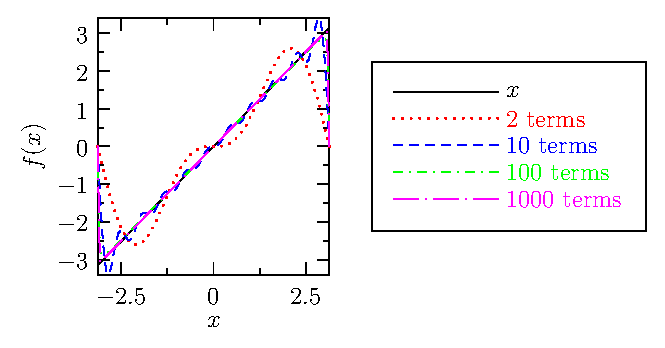
\includegraphics{figures/fourierx}
      }{
        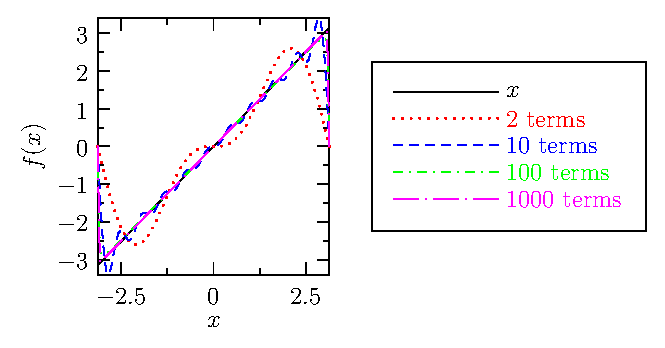
\includegraphics[width=\textwidth]{figures/fourierx}
      }
      %FIXME: is this the correct width for the normal figure?
      \caption{Fourier series approximations to $f(x)=x$.}
      \label{fourierx}
    \end{center}
  \end{figure}
}

%TODO: something about orthogonality? More examples?

\newpage
\section{Problems}

\begin{enumerate}
  \item
    What are the Fourier sine and cosine series for
    $y=\sin x$, $x \in (-\pi,\pi)$?
    \hidesolution{
      Students should make use of the orthogonality property for $\sin nx$ and
      $\sin mx$, $n \neq m$.
    }
  \item
    What is the Fourier series for $ f(x) = \d(x-1)$, $x \in (-\pi,\pi)$?
  \item
    What is the Fourier series for $ f(x) = 2 u_0(t)-1 $, $x \in (-\pi,\pi)$?

  \item What is the Fourier series in $x$ for $f(x,t)$, $x \in (-\pi,\pi)$, if
    \begin{dmath*}[compact]
      f(x,t) =
      \left\{ \begin{array}{ll}
        -t           & \mbox{if $x < 0$};\\
        \phantom{-}t & \mbox{if $x \geq 0$}
      \end{array} \right. ?
    \end{dmath*}

\end{enumerate}


\chapter{Partial Differential Equations:
         \\Actually Solving Them}
\ifthenelse{\value{small}=1}{\newpage}

Let us now return to the heat equation,
\begin{eqnarray}
  \label{heateq}
  \pp{u}{t} = \beta \pptwo{u}{x},
\end{eqnarray}
and add some \emph{initial conditions}
\begin{dmath*}
  u(x,0)=f(x),
\end{dmath*}
and \emph{boundary conditions}
\begin{eqnarray}
  \label{homdibc}
  u(0,t)=0, \qquad u(\pi,t)=0.
\end{eqnarray}
Physically, this corresponds to modelling the temperature on a rod of
length $\pi$ in contact at both ends with a heat sink with temperature
$0$ (note that this is not necessarily absolute zero: if we take
$u=u+C$, the equation remains the same, so our base temperature is
arbitrary.) The rod starts with the temperature at position $x$ given
by $f(x)$.

We'll solve this using separation of variables:
\begin{eqnarray}
  \label{heatF}
  u = \sum_{n=0}^\infty T_n(t) X_n(x),
\end{eqnarray}
where we have taken $X_n(x)$ to be orthogonal\footnote{That is, if
  $i\neq j$, then $\int_0^\pi X_i(x) X_j(x) dx =0.$ This is the case
  with elements of $\{1,\cos(nx),\sin(nx),n=1,2,\dots \}$.}.  Putting
equation~\eqref{heatF} into equation~\eqref{heateq}, we get
\begin{eqnarray}
  \label{heats}
  \sum_{n=0}^\infty \ddt{T_n(t)}X_n(x)
  =\beta\sum_{n=0}^\infty T_n(t)\ddtwo{X_n(x)}{x}
\end{eqnarray}
Now, since the $X_n$'s are orthogonal, this actually holds term-by-term. That
is, for each $n$, we have
\begin{dmath*}
  T_n'(t)X_n(x) = \beta  T_n(t)X_n''(x)
\end{dmath*}
which we can rearrange to get
\begin{dmath*}
  \frac{1}{\beta}\frac{T_n'(t)}{T_n(t)}= \frac{X_n''(x)}{X_n(x)}.
\end{dmath*}
Now, the LHS is independent of $x$, so the RHS must also be independent of $x$.
Since the RHS is also clearly independent of $t$, it must be constant. That is,
\begin{dmath*}[compact]
  \boxed{
    \frac{1}{\beta}\frac{T_n'(t)}{T_n(t)}
    = \frac{X_n''(x)}{X_n(x)} 
    = K_n,
  }
\end{dmath*}
where $K_n$ can only depend on $n$.

This gives us an ODE for $X_n$,
\begin{eqnarray}
  \label{Eigenfunction}
  \boxed{X_n'' = K_n X_n.}
\end{eqnarray}
Now, depending on the sign of $K_n$, we have three possibilities, which we will
deal with by enforcing the boundary conditions. Since the $X_n$ are orthogonal,
the boundary conditions must be satisfied for each $n$. The cases are:
\begin{enumerate}
  \item $K_n=k_n^2 > 0$. In this case, $X_n(x)= C_1 \cosh(k_n x) +C_2
    \sinh(k_n x)$.  But then, $X_n(0)=0$ implies that $C_1=0$, and
    $X_n(\pi)=0$ implies that $C_2=0$, so this eigenfunction is zero.
  \item $K_n = 0$. In this case, we get $X_n(x)=C_1 +C_2 x$. Again,
    the boundary conditions imply that $C_1=C_2=0$, so this
    eigenfunction is again zero.
  \item $K_n =-k_n^2 < 0$. This gives us periodic behaviour,
    \begin{dmath*}
      X_n(x)=C_1\cos(k_nx) + C_2\sin(k_nx).
    \end{dmath*}
    We require that $X_n(0)=C_1=0$, so we can remove all the cosines. The
    other boundary condition gives us
    \begin{dmath*}[compact]
      X_n(\pi)=C_2\sin(k_n\pi)=0,
    \end{dmath*}
    which implies that either $C_2=0$ or $k_n$ is an integer. Since this is
    our last chance to have $X_n$ not be zero everywhere, we can't have $C_2=0$,
    so we set $k_n$ to be an integer. In particular, set $k_n=n$.
\end{enumerate}
Thus, $K_n=-n^2$, and 
\begin{dmath*}
  \boxed{X_n= \sin(nx).}
\end{dmath*}
Much simpler!

We now have enough information to start determining $T_n$. We know that
$K_n=-n^2$, so $T_n$ obeys the equation
\begin{dmath*}[compact]
  T_n' = \beta K_n T_n = - \beta n^2 T_n
\end{dmath*}
which is solved by
\begin{dmath*}[compact]
  \boxed{T_n = T_n(0) e^{-\beta n^2 t}.}
\end{dmath*}

Putting this together, our solution (so far) is
\begin{dmath*}
  u(x,t) = \sum_{n=0}^\infty T_n(0) e^{-\beta n^2 t} \sin(nx).
\end{dmath*}
To get this, we have used the original equation and the boundary conditions.
We still have to determine the values of $T_n(0)$, for which we will use the
initial conditions, $u(x,0)=f(x)$. That is,
\begin{dmath*}
  u(x,0)=f(x) 
  =  \sum_{n=0}^\infty T_n(0) e^{-\beta n^2 t} \sin(nx)
  = \sum_{n=0}^\infty T_n(0) \sin(nx).
\end{dmath*}
In other words, this is just a sine-series for $f(x)$! However, instead of
integrating over $(-\pi,\pi)$, we only know $f(x)$ for $x\in(0,\pi)$. We can
solve this problem by extending $f(x)$ as an odd function by setting
$f(-x)=-f(x)$, so the coefficients are given by
\begin{dmath*}
  T_n(0)=\frac{1}{\pi}\int_{-\pi}^\pi f(x)\sin(nx)dx
  =\frac{2}{\pi}\int_0^\pi f(x)\sin(nx)dx,
\end{dmath*}
since the integrand is even.

The solution to the heat equation, for the type of initial and
boundary conditions given above, is
\begin{dmath*}
\boxed{
    u(x,t)=\frac{2}{\pi}
    \sum_{n=1}^\infty \[\int_0^\pi f(x)\sin(nx)\,dx\]
    e^{-kn^2t}
    \sin(nx) 
  .}
\end{dmath*}

\workedexample{
  The initial temperature in a rod of length $\pi$ is given by
  \begin{eqnarray}
    \label{heat1ic}
    u(x,0)=2\sin(x)+\sin(5x),
  \end{eqnarray}
  and the temperature at the ends of the rod is kept at zero. Assuming that
  \begin{dmath*}
    \pp{u}{t} = \beta\pptwo{u}{x},
  \end{dmath*}
  find $y(x,t)$ for $x\in(0,\pi)$, $t>0$.
  }\\
{
  The boundary conditions match those given in equation~\eqref{homdibc}, so
  the above analysis shows that we can express $y$ as a linear combination
  of $\{\sin(nx),n=1,2,\dots\}$. That is,
  \begin{dmath*}
    u(x,t)=\sum_{n=1}^\infty T_n(0) e^{-\b n^2 t} \sin(nx).
  \end{dmath*}
  The initial conditions are that $y(x,0)=2\sin(x)+\sin(5x)$, so $T_1(0)=2$,
  $T_5(0)=1$, and all others are zero. We can then write the solution as
  \begin{dmath*}
    u(x,t) = 2 e^{-\b t} \sin(x) + e^{-25 \b t} \sin(5x).
  \end{dmath*}
%FIXME: Is this enough explanation?
 This result is shown for various times in figure \ref{heat1} for $\b=1$.
  \begin{figure}[htbp]
    \begin{center}
      \ifthenelse{\value{small}=0}{
        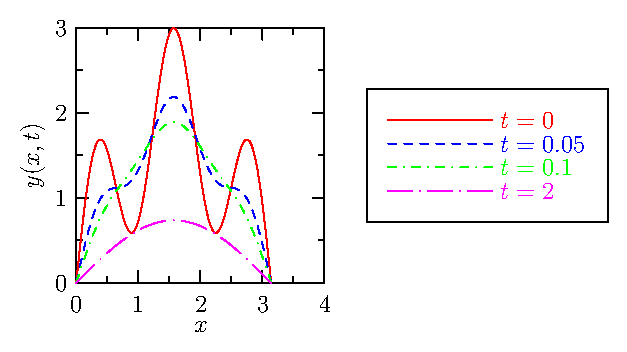
\includegraphics{figures/heat1}
      }{
        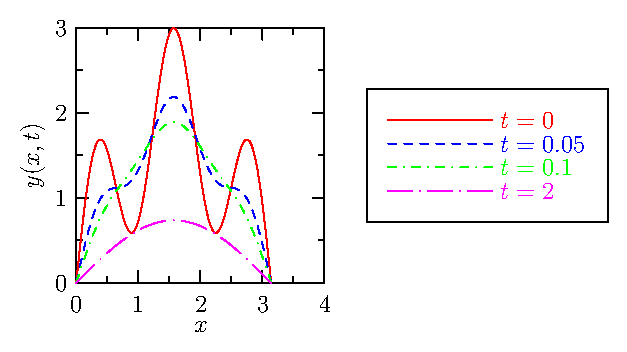
\includegraphics[width=\textwidth]{figures/heat1}
      }
      %FIXME: is this figure too wide for letter-size pages?
      \caption{The temperature at different times with initial
        conditions given in equation~\eqref{heat1ic}. Notice that the
        $\sin(5x)$ term, which decays like $e^{-25 \b t}$, is relevant
        only for small $t$. }
      \label{heat1}
    \end{center}
  \end{figure}
}


\section{Non-homogeneous constant boundary conditions}

Suppose that the boundary conditions were instead
\begin{dmath*}[compact]
  u(0,t)=A, \qquad u(\pi,t)=B.
\end{dmath*}
Notice that these conditions match the case $K_n=0$ with
\begin{dmath*}
  u(x,t)=\frac{B-A}{\pi}x+A.
\end{dmath*}
This obeys the heat equation, since
\begin{dmath*}[compact]
  \pptwo{}{x}(mx+b)=0= \pp{}{t}(mx+b),
\end{dmath*}
and is independent of $t$, i.e.\ it is a steady state solution. Then, setting
\begin{dmath*}
  g(x) = f(x) - \(A+ \frac{B-A}{\pi}x\),
\end{dmath*}
\begin{dmath}
  \label{diribc}
  u(x,t)=A + \frac{B-A}{\pi}x +
  \frac{2}{\pi}
  \sum_{n=1}^\infty\(\int_{0}^\pi g(x)\sin(nx)dx\) e^{-\b n^2t} \sin(nx)
\end{dmath}
matches both the initial and boundary conditions.

\workedexample{
  Solve the initial boundary problem
  \begin{dmath}
    \label{heat3ic}
    \pp{u}{t} \no{=} \b \pptwo{u}{x},
  \end{dmath}
  \begin{dmath*}
    \qquad u(0)\no{=}1, \quad u(\pi)\no{=}1\no{+}\pi,
  \end{dmath*}
  \begin{dmath*}
    \quad u(x,0)\no{=}f(x)\no{=}x^2 +x +1
  \end{dmath*}
  for $u(x,t)$.

}{
  The steady-state solution is $x+1$. Let
  \begin{dmath*}
    g(x) = f(x) -(x+1) = x^2
  \end{dmath*}
  Then,
  \begin{dmath*}
    u(x,t) = 1 + x + \sum_{n=1}^\infty T_n(0) e^{-\b n^2 t} \sin(nx).
  \end{dmath*}
  And in order to satisfy $y(x,0)=1+x+x^2$, we have
  \begin{dmath*}
    x^2 = \sum_{n=1}^\infty T_n(0) \sin(nx).
  \end{dmath*}
  The coefficients are given by the formula
  \begin{dmath*}
    T_n(0) 
    = \frac{2}{\pi} \int_0^\pi x^2 \sin(nx) \, dx
    = \frac{2}{\pi}\[\left.x^2 \frac{-\cos(nx)}{n} \right|_0^\pi
    + \frac{2}{n}\int_0^\pi x \cos(nx)dx\]
    = \frac{2}{n\pi}\[ -\pi^2\cos(n\pi)+2(\left.\frac{x \sin(nx)}{n}
    \right|_0^\pi
    - \frac{1}{n}\int_0^\pi\sin(nx)dx)  \]
    = \frac{-2\pi}{n}\cos(n\pi)-\frac{4}{n^3\pi} \left.-\cos(nx) \right|_0^\pi
    = \frac{-2\pi}{n}(-1)^n + \frac{4(\(-1)^n-1\)}{n^3\pi}
  \end{dmath*}
  The solution is therefore
  \begin{dmath*}
    u(x,t) = 1+x+
    \sum_{n=1}^\infty \[\frac{-2\pi}{n}(-1)^n + \frac{4(\(-1)^n-1\)}{n^3\pi}\]
    e^{-\b n^2 t}\sin(nx).
  \end{dmath*}
% Useless figure
%  as can be seen in figure \ref{heat3}. \qed
%  \begin{figure}[htbp]
%    \begin{center}
%      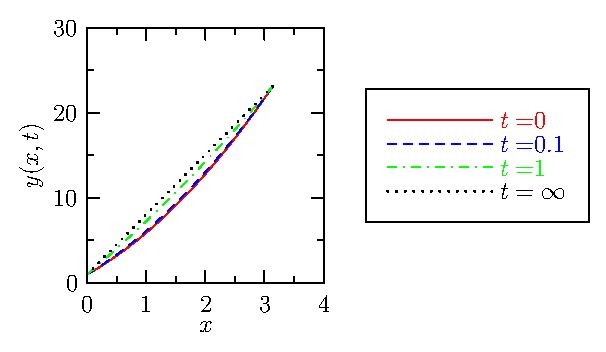
\includegraphics{figures/heat3}
%      \caption{The temperature at different times for the system given in
%        \eqref{heat3ic}.}
%      \label{heat3}
%    \end{center}
%  \end{figure}

}
% This lab is too long!
%\section{A more complicated example}
%
%\workedexample{
%  The heat in a rod obey the equation
%  \be
%  \pp{y}{t}=\pptwo{y}{x}.
%  \ee
%  Given the boundary conditions
%  \be
%  \label{heat2ic}
%  y(0,t)=1 \qquad y(\pi,t)=e^\pi
%  \ee
%  and the and the initial condition $y(x,0)=e^x$, find $y(x,t)$.\\
%}{
%  The solution is given by
%  \be
%  y(x,t)&=&1 + \frac{e^\pi-1}{\pi}x +
%  \sum_{n=1}^\infty T_n(0) e^{-n^2t} \sin(nx),
%  \\
%  T_n(0)&=&\frac{2}{\pi}\int_{0}^\pi g(x)\sin(nx)dx,
%  \\
%  g(x)&=&e^x - 1 - \frac{e^\pi-1}{\pi}x.
%  \ee
%  From equation~\eqref{Fourierx}, we have
%  \be
%  x = 2 \sum_{n=1}^\infty  \frac{(-1)^{n+1}}{n} \sin(nx)
%  \ee
%  To find the Fourier sine-series for $e^x$, we must compute
%  \be
%  a_n = \frac{2}{\pi}\int_0^\pi e^x \sin(nx) \, dx
%  = \frac{2}{\pi}\left.\frac{e^x\(\sin(nu) - n \cos(nu)\)}{n^2+1}\right|_0^\pi
%  = \frac{2}{\pi}\frac{n(1 - (-1)^ne^\pi)}{n^2+1}
%  \ee
%  Also, the Fourier series for $1$ over $x\in(-\pi,\pi)$ has coefficients
%  \be
%  \frac{2}{\pi}\int_0^\pi \sin(nx) = \frac{2}{n\pi}\left.\cos(nx) \right|_0^\pi
%  = \frac{2\((-1^n)-1\)}{n\pi},
%  \ee
%  so, over $x\in(0,\pi)$,
%  \be
%  1 = \sum_{n=1}^\infty \frac{2\((-1^n)-1\)}{n\pi} \sin(nx).
%  \ee
%
%  Noting that the Fourier series is a linear, so we can add the series
%  together:
%  \be
%  e^x - 1- \frac{e^\pi}{\pi}x
%  &=& \sum_{n=1}^\infty \frac{2}{\pi}n\frac{1 - (-1)^ne^\pi}{n^2+1} \sin(nx)
%  - \frac{e^\pi-1}{\pi} 2 \sum_{n=1}^\infty  \frac{(-1)^{n+1}}{n} \sin(nx)
%  \\ \nonumber
%  &&-\sum_{n=1}^\infty \frac{2\((-1^n)-1\)}{n\pi} \sin(nx)
%  \\ \nonumber
%  &=&\sum_{n=1}^\infty \(\frac{2}{\pi}\frac{n(1 - (-1)^ne^\pi)}{n^2+1}
%  -\frac{e^\pi-1}{\pi}2 \frac{(-1)^{n+1}}{n}- \frac{2\((-1^n)-1\)}{n\pi}\)
%  \sin(nx).
%  \ee
%  Now, this is all a bit messy, but we do end up with the solution
%  \be
%  y(x,t) = 1 &+& \frac{e^\pi-1}{\pi}x
%  \\ \nonumber
%  &+&
%  \sum_{n=1}^\infty \(\frac{2}{\pi}\frac{n(1 - (-1)^ne^\pi)}{n^2+1}
%  -2 \frac{e^\pi-1}{\pi} \frac{(-1)^{n+1}}{n}- \frac{2\((-1^n)-1\)}{n\pi}\)
%    e^{-n^2t} \sin(nx),
%  \ee
%  as can be seen in figure \ref{heat2}. \qed
%  \begin{figure}[htbp]
%    \begin{center}
%      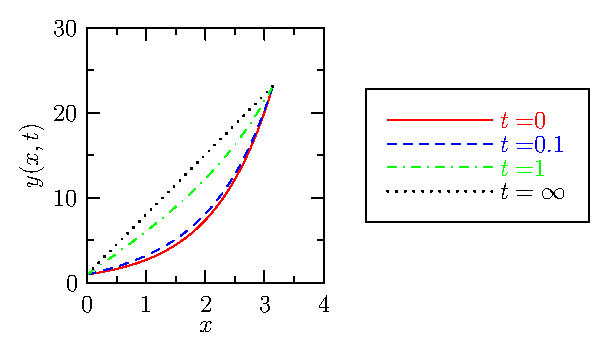
\includegraphics{figures/heat2}
%      \caption{The temperature at different times with initial conditions
%        given in \eqref{heat2ic}.}
%      \label{heat2}
%    \end{center}
%  \end{figure}
%}


\newpage
\ifthenelse{\value{small}=1}{
  \subsection{Flow chart for the heat eqn.}
}{
  \subsection{Flow chart for solving the heat equation}
}
%FIXME: text

%FIXME: refer to this somewhere
\vspace{0.5in}
\begin{figure}[!h]
  \centering
\ifthenelse{\value{small}=1}{
  \includegraphics[width=0.9\textwidth]{figures/heatsepflow}
}{
  \includegraphics[width=\textwidth]{figures/heatsepflow}
}
  \caption{Flow chart for solving the heat equation.}
  \label{fig:heatsepflow}
\end{figure}

\newpage
\section{Problems}

\begin{enumerate}
  \item
    Show that equation~\eqref{diribc} does indeed solve the heat equation
    with the given boundary and initial conditions.
  \item
    Solve the heat equation 
    \begin{dmath*}
      \pp{u}{t} = \beta \pptwo{u}{x}
    \end{dmath*}
    with boundary conditions $u(0,t)=u(\pi,t)=0$ and initial condition
    $u(x,0)=2\sin(x) - \sin(3x)$.
  \item
    An inanimate carbon rod of length $\pi$ is hit with a ``laser'',
    transferring an amount of heat $H$ to a point at its centre, where
    $H$ is a constant. That is, the initial temperature distribution
    along its length is given by
    \begin{dmath*}
      u(x,0)=H\delta\(x-\frac{\pi}{2}\).
    \end{dmath*}
    If the ends of the rod are kept at constant temperature $0$, and the
    temperature in the rod obeys the relationship
    \begin{dmath*}
      \pp{u}{t} = \beta \pptwo{u}{x}
    \end{dmath*}
    find $u(x,t)$ for all $t\geq 0$.
    \hidesolution{
      Following the above procedure,
      \begin{dmath*}
        u(x,t)=\frac{2}{\pi}\sum_{n=1}^\infty T_n(0) e^{-kn^2t} \sin(nx)
      \end{dmath*}
      with
      \begin{dmath*}
        T_n(0) 
        = \frac{2}{\pi}\int_0^\pi H \d\(x-\frac{\pi}{2} \) \sin(nx) \, dx
        = \frac{2H}{\pi} \sin\(\frac{n\pi}{2}\)
        = \frac{2H}{\pi}
        \left\{ \begin{array}{ll}
          0,           & \mbox{if $n=2m$}\\
          \sin\(m\pi+ \frac{\pi}{2}\), & \mbox{if $n=2m+1$}
        \end{array} \right.
        = \frac{2H}{\pi}
        \left\{ \begin{array}{ll}
          0,           & \mbox{if $n=2m$}\\
          (-1)^m, & \mbox{if $n=2m+1$}.
        \end{array} \right.
      \end{dmath*}
      The solution is then given by
      \begin{dmath*}
        u(x,t) 
        = \frac{2H}{\pi} \sum_{m=0}^\infty (-1)^m e^{-4\beta m^2 t} \sin(2mx)
      \end{dmath*}
    }
  \item
    %\emph{Dirichlet boundary conditions} specify the value of the
    %function at the boundary, e.g.\ $u(0,t)=A$, $u(\pi,t)=B$ with $A$
    %and $B$ constant.  We showed that the set of Eigenfunctions given
    %by equation~\eqref{Eigenfunction} must be
    %$\{\sin(nx),n=1,2,\dots\}$ in this case.
    % 
    If the boundary conditions were instead 
    \emph{homogeneous Neumann boundary conditions} at $x=0$ and $x=\pi$,
    \begin{dmath*}[compact]
    \left.\pp{u(x,t)}{x}\right|_{x=0}=0, \qquad
        \left.\pp{u(x,t)}{x}\right|_{x=\pi}=0,
    \end{dmath*}
    and the initial condition
    $u(x,0)=\cos(x)$, what is the solution to the heat equation,
    $\ppt{u}=\b \pptwo{u}{x}$?
    \hidesolution{ 
      The first step is separation of variables: let $u(x,t)=\sum_\a
      T_\a(t) X_\a(x)$. We take a single mode, $T_\a X_\a$, and put it 
      into the PDE,
      $$
      \ppt{T_\a X_\a} = \b \pptwo{T_\a X_\a}{x}
      \quad \implies \quad
      \frac{1}{\b} \frac{T'_\a}{T_\a} = \frac{X^{''}_\a}{X_\a} =\a
      $$
      Solving for $T_\a$ we get $T_\a(t)=T_\a(0)e^{\a\b t}$. Solving
      for $X_\a$ is more complicated, as there are three cases:
      \begin{enumerate}
        \item $\a = \l^2 > 0$:
          In this case we get $X_\a = C_1 \cosh (\l x) + C_2 \sinh(\l x)$.
          To match the boundary conditions, we need
          $X^'_\a=\l C_1 \sinh(\l x) + \l C_2 \cosh(\l x)$.
          Applying the first boundary condition,
          $$
          X^'_\a(0)=\l C_2 =0  \quad \implies \quad C_2 =0,
          $$
          so $X_\a = \l C_1 \cosh(\l x)$.
          Applying the second boundary condition gives 
          $$
          X^'_\a(\pi) = \l C_1 \sinh(\l \pi)=0.
          $$
          Since $ \l \sinh(\l \pi)\neq 0$, we conclude that $C_1=0$, 
          and that this mode is trivial.

        \item $\a=0$:
          In this case $X_\a = C_1 + C_2 x$, and $X^'_\a=C_2$. Then 
          the left boundary condition gives
          $$
          X^'_\a(0)=C_2=0
          $$
          and the right boundary condition gives us the same thing:
          $$
          X^'_\a(\pi)=C_2=0.
          $$ 
          Let's use $a_0/2$ instead of $C_1$, and we're left with
          $X_\a=a_0/2$, a constant.

        \item $\a=-\l^2 < 0$:
          In this case $X_\a=C_1 \cos(\l x) + C_2 \sin(\l x)$, and
          $X^'_\a=-C_1 \l \sin(\l x) + C_2 \l \cos(\l x)$.
          The left boundary condition implies that
          $$
          X^'_\a(0)=C_2 \l =0
          $$
          and, since $\l\neq 0$ in this case, we get $C_2=0$, so that
          $X_\a = C_1 \cos(\l x)$. the right boundary condition implies that
          $$
          X^'_\a(\pi)=-C_1 \l \sin(\l \pi) =0
          $$
          which implies that either $C_1=0$ or $\sin(\l \pi)=0$. This second 
          case happen when $\l \pi = n \pi$, i.e.\ $\l=n$. Thus, the
          non-trivial modes for this case are 
          $$
          X_\a = C_2 \cos(n x).
          $$

      \end{enumerate}
      Having determined all the modes $T_\a X_\a$, we can put them into
      the series solution for $u$, which is
      $$
      u(x,t) = \frac{a_0}{2} + \sum_{n=1}^\infty a_n e^{-\b n^2 t} \cos(n x) .
      $$
      The initial conditions are $u(x,0)=\cos(x)$, so
      $$
      u(0,t) = \frac{a_0}{2} + \sum_{n=1}^\infty a_n  \cos(n x) = \cos(x),
      $$
      which is a Fourier cosine series for $\cos(x)$.  We could
      use the formula for cosine series to calculate $a_n$, but, since
      $\cos(x)$ is already a Fourier cosine series, we can just match
      term-by-term, getting $a_1=1$, and $a_n=0$ if $n\neq 1$. The 
      solution is then
      \begin{dmath*}
        u(x,t) 
        = e^{-\b 1^2 t} \cos(1 x) 
        = e^{-\b  t} \cos(x).
      \end{dmath*}
    }


\end{enumerate}


\appendix{}
\chapter{Tables}
\ifthenelse{\value{small}=1}{\newpage}



\section{Table of Taylor Series}

\ifthenelse{\value{small}=0}{

$$
\begin{tabular}{ l |  l }
  $f(t)$ & $\Laplace(f) = F(s)$  \\
  \hline
  \hline
  \multirow{2}{*}{$ f'(t)$}
  & \multirow{2}{*}{$sF(s) -f(0)$} \\ \\ \hline
  \multirow{2}{*}{$f''(t)$}
  & \multirow{2}{*}{$s^2F(s) -sf(0) - f'(0)$} \\ \\ \hline
  \multirow{2}{*}{$ f^{(n)}(t)$}
  & \multirow{2}{*}{$ s^nF(s) -s^{n-1}f(0)-\dots - f^{(n-1)}(0)$}\\ \\ \hline
%  \multirow{2}{*}{$\displaystyle t$}                                           
%  & \multirow{2}{*}{$\displaystyle\frac{1}{s^2}$} \\ \\ \hline                 
  \multirow{2}{*}{$\displaystyle t^n$}
  & \multirow{2}{*}{$\displaystyle\frac{n!}{s^{n+1}}$} \\ \\ \hline
  \multirow{2}{*}{$\displaystyle e^{\a t}$ }
  & \multirow{2}{*}{$\displaystyle\frac{1}{s-\a} $} \\ \\ \hline
  \multirow{2}{*}{$e^{\a t}f(t) $}
  & \multirow{2}{*}{$ F(s-\a) $} \\  \\ \hline
  \multirow{2}{*}{$\displaystyle f(ct) $ }
  & \multirow{2}{*}{$\displaystyle \frac{1}{c}F\(\frac{s}{c}\) $} \\ \\ \hline
  \multirow{2}{*}{$\displaystyle \cos(\b t)$}
  & \multirow{2}{*}{$\displaystyle \frac{s}{s^2 + \b^2} $} \\ \\ \hline
  \multirow{2}{*}{$\displaystyle \sin(\b t)$}
  & \multirow{2}{*}{$\displaystyle \frac{\b}{s^2 + \b^2} $} \\ \\ \hline
  \multirow{2}{*}{$\displaystyle \cosh(\b t)$}
  & \multirow{2}{*}{$\displaystyle \frac{s}{s^2 - \b^2}$} \\ \\ \hline
  \multirow{2}{*}{$\displaystyle \sinh(\b t)$ }
  & \multirow{2}{*}{$\displaystyle \frac{\b}{s^2 - \b^2} $} \\ \\ \hline
  \multirow{2}{*}{$\displaystyle e^{\a t}\cos(\b t)$}
  & \multirow{2}{*}{$\displaystyle \frac{s-\a}{(s-\a)^2 + \b^2}$} \\ \\ \hline
  \multirow{2}{*}{$\displaystyle e^{\a t}\sin(\b t)$}
  & \multirow{2}{*}{$\displaystyle \frac{\b}{(s-\a)^2 + \b^2}$} \\ \\ \hline
  \multirow{2}{*}{$\displaystyle u_c(t)$, $c > 0$}
  & \multirow{2}{*}{$\displaystyle {e^{-cs}}/{s}$} \\ \\ \hline
  \multirow{2}{*}{$u_c(t)f(t-c)$, $c > 0$}
  & \multirow{2}{*}{$e^{-cs}F(s)$} \\  \\ \hline
  \multirow{2}{*}{$\delta(t-c)$, $c > 0$}
  & \multirow{2}{*}{$e^{-cs}$} \\  \\ \hline
  \multirow{2}{*}{$\displaystyle \int_0^t f(t-\t)g(\t) \,d\t \doteq f*g$}
  & \multirow{2}{*}{$\displaystyle F(s)G(s)$} \\ \\ \hline
  \multirow{3}{*}{$\displaystyle f(t)$ with $\displaystyle f(t+T)=f(t)$}
  & \multirow{3}{*}{$\displaystyle \frac{\int_0^Tf(t) e^{-st}dt}{1-e^{-sT}}$}
  \\ \\ \\ \hline
  \multirow{2}{*}{$\displaystyle t^n f(t)$}
  & \multirow{2}{*}{$\displaystyle (-1)^n \frac{d^n}{ds^n} F(s)$} \\ \\ \hline
\end{tabular}\\
$$
}{ % the table doesn't work very well here; just list the Taylor series.
\begin{dmath*}
  f(x) = f(a) + f'(a)(x-a) + \frac{f''(a)}{2!} + \dots
  + \frac{f^{(n)}(a)}{n!}(x-a)^n + \dots
\end{dmath*}
\begin{dmath*}
  e^x = \sum_{n=0}^\infty \frac{x^n}{n!}
\end{dmath*}
\begin{dmath*}
  \sin x = \sum_{n=0}^\infty \frac{(-1)^n x^{2n+1}}{(2n+1)!}
\end{dmath*}
\begin{dmath*}
  \sin x = \sum_{n=0}^\infty \frac{(-1)^n x^{2n+1}}{(2n+1)!}
\end{dmath*}
\begin{dmath*}
  \tan x = x + \frac{1}{3}x^3 + \frac{2}{15}x^5 + \frac{17}{315}x^7
  + \frac{62}{2835}x^9 + \dots
\end{dmath*}
\begin{dmath*}
  \arcsin x = x + \frac{1}{2}\frac{x^3}{3}
  + \frac{1\cdot 3}{2\cdot 4}\frac{x^5}{5}
  + \frac{1\cdot3\cdot5}{2\cdot4\cdot6}\frac{x^7}{7} + \dots
\end{dmath*}
\begin{dmath*}
  \arctan x = \sum_{n=0}^\infty (-1)^n \frac{x^{2n+1}}{2n+1}
\end{dmath*}
\begin{dmath*}
  \frac{1}{1-x} = \sum_{n=0}^\infty x^n
\end{dmath*}
\begin{dmath*}
  \ln(1-x) = -\sum_{n=1}^\infty \frac{x^n}{n}
\end{dmath*}
}
\newpage
\section{Table of Laplace Transforms}

%FIXME: this isn't formatting right
\label{sec:tableolap}
$$
\begin{tabular}{ l |  l }
  $f(t)$ & $\Laplace(f) = F(s)$  \\
  \hline
  \hline
  \multirow{2}{*}{$ f'(t)$}
  & \multirow{2}{*}{$sF(s) -f(0)$} \\ \\ \hline
  \multirow{2}{*}{$f''(t)$}
  & \multirow{2}{*}{$s^2F(s) -sf(0) - f'(0)$} \\ \\ \hline
  \multirow{2}{*}{$ f^{(n)}(t)$} 
  & \multirow{2}{*}{$ s^nF(s) -s^{n-1}f(0)-\dots - f^{(n-1)}(0)$}\\ \\ \hline
%  \multirow{2}{*}{$\displaystyle t$}
%  & \multirow{2}{*}{$\displaystyle\frac{1}{s^2}$} \\ \\ \hline
  \multirow{2}{*}{$\displaystyle t^n$}
  & \multirow{2}{*}{$\displaystyle\frac{n!}{s^{n+1}}$} \\ \\ \hline
  \multirow{2}{*}{$\displaystyle e^{\a t}$ }
  & \multirow{2}{*}{$\displaystyle\frac{1}{s-\a} $} \\ \\ \hline
  \multirow{2}{*}{$e^{\a t}f(t) $}
  & \multirow{2}{*}{$ F(s-\a) $} \\  \\ \hline
  \multirow{2}{*}{$\displaystyle f(ct) $ }
  & \multirow{2}{*}{$\displaystyle \frac{1}{c}F\(\frac{s}{c}\) $} \\ \\ \hline
  \multirow{2}{*}{$\displaystyle \cos(\b t)$}
  & \multirow{2}{*}{$\displaystyle \frac{s}{s^2 + \b^2} $} \\ \\ \hline
  \multirow{2}{*}{$\displaystyle \sin(\b t)$}
  & \multirow{2}{*}{$\displaystyle \frac{\b}{s^2 + \b^2} $} \\ \\  \hline
\ifthenelse{\value{small}=1}{ % end table here for small page-size 
\end{tabular} 
$$

$$
\begin{tabular}{ l |  l }
  $f(t)$ & $\Laplace(f) = F(s)$  \\
  \hline
  \hline 
}{}
  \multirow{2}{*}{$\displaystyle \cosh(\b t)$}
  & \multirow{2}{*}{$\displaystyle \frac{s}{s^2 - \b^2}$} \\ \\ \hline
  \multirow{2}{*}{$\displaystyle \sinh(\b t)$ }
  & \multirow{2}{*}{$\displaystyle \frac{\b}{s^2 - \b^2} $} \\ \\ \hline
  \multirow{2}{*}{$\displaystyle e^{\a t}\cos(\b t)$}
  & \multirow{2}{*}{$\displaystyle \frac{s-\a}{(s-\a)^2 + \b^2}$} \\ \\ \hline
  \multirow{2}{*}{$\displaystyle e^{\a t}\sin(\b t)$}
  & \multirow{2}{*}{$\displaystyle \frac{\b}{(s-\a)^2 + \b^2}$} \\ \\ \hline
  \multirow{2}{*}{$\displaystyle u_c(t)$, $c > 0$}
  & \multirow{2}{*}{$\displaystyle {e^{-cs}}/{s}$} \\ \\ \hline
  \multirow{2}{*}{$u_c(t)f(t-c)$, $c > 0$}
  & \multirow{2}{*}{$e^{-cs}F(s)$} \\  \\ \hline
  \multirow{2}{*}{$\delta(t-c)$, $c > 0$} 
  & \multirow{2}{*}{$e^{-cs}$} \\  \\ \hline
  \multirow{2}{*}{$\displaystyle \int_0^t f(t-\t)g(\t) \,d\t \doteq f*g$} 
  & \multirow{2}{*}{$\displaystyle F(s)G(s)$} \\ \\ \hline
  \multirow{3}{*}{$\displaystyle f(t)$ with $\displaystyle f(t+T)=f(t)$}
  & \multirow{3}{*}{$\displaystyle \frac{\int_0^Tf(t) e^{-st}dt}{1-e^{-sT}}$}
  \\ \\ \\ \hline
  \multirow{2}{*}{$\displaystyle t^n f(t)$}
  & \multirow{2}{*}{$\displaystyle (-1)^n \frac{d^n}{ds^n} F(s)$} \\ \\ \hline
\end{tabular}\\
$$



\newpage
\section{Table of Integrals}
\begin{dmath*}
  \int u dv = uv - \int v du
\end{dmath*}  
\begin{dmath*}
   \int \cos x dx = -\sin x
\end{dmath*}  
\begin{dmath*}
   \int \sin x dx = \cos x
\end{dmath*}  
\begin{dmath*}
   \int \tan x dx  = -\ln\abs{\cos x}
\end{dmath*}  
\begin{dmath*}
   \int \sin^2 x dx = \frac{1}{2}x - \frac{1}{4}\sin 2x
\end{dmath*}  
\begin{dmath*}
   \int \cos^2 x dx = \frac{1}{2}x + \frac{1}{4}\sin 2x
\end{dmath*}  
\begin{dmath*}  
   \int \tan^2 x dx  = \tan x - x
\end{dmath*}  
\begin{dmath*}
    \int \sin^n x dx = -\frac{\sin^{n-1}x\cos{x}}{n}
  + \frac{n-1}{n}\int\sin^{n-2}xdx
\end{dmath*}  
\begin{dmath*}  
   \int \cos^n x dx = \frac{\cos^{n-1}x\sin x}{n}
  + \frac{n-1}{n}\int \cos^{n-2}x dx
\end{dmath*}  
\begin{dmath*}
   \int \sin ax \sin bx dx = - \frac{\sin(a+b)x}{2(a+b)}
  + \frac{\sin(a-b)x}{2(a-b)},\\a^2\no\neq b^2
\end{dmath*}  
\begin{dmath*}
   \int \cos ax \cos bx dx = \frac{\sin(a+b)x}{2(a+b)}
  + \frac{\sin(a-b)x}{2(a-b)},\\ a^2\no\neq b^2
\end{dmath*}  
\begin{dmath*}
   \int \sin ax \cos bx dx = -\frac{\cos(a+b)x}{2(a+b)}
  - \frac{\cos(a-b)x}{2(a-b)},\\ a^2\no\neq b^2
\end{dmath*}  
\begin{dmath*}
   \int \sec^2 x dx = \tan x
\end{dmath*}  
\begin{dmath*}
   \int \csc^2 x dx = -\cot x
\end{dmath*}  
\begin{dmath*}
   \int \sec x \tan x  dx = \sec x
\end{dmath*}  
\begin{dmath*}
   \int \frac{dx}{\sqrt{a^2-x^2}}= \arcsin\frac{x}{a}
\end{dmath*}  
\begin{dmath*}
  \int \frac{dx}{x\sqrt{x^2-a^2}}= \frac{1}{a}\arccos\frac{a}{x}
\end{dmath*}  
\begin{dmath*}
  \int \frac{dx}{a^2+x^2} = \frac{1}{a}\arctan\frac{x}{a},
\end{dmath*}  
\begin{dmath*}
   \int \frac{dx}{a^2-x^2} = \frac{1}{2a}\ln\abs{\frac{x+a}{x-a}},
\end{dmath*}  
\begin{dmath*}
   \int \frac{dx}{\sqrt{a^2+x^2}} = \ln\abs{x+\sqrt{x^2+a^2}}
\end{dmath*}  
\begin{dmath*}
   \int \sinh x dx = \cosh x
\end{dmath*}  
\begin{dmath*}
   \int \cosh x dx = \sinh x
\end{dmath*}  
\begin{dmath*}
  \int e^{ax}\sin nx dx = \frac{e^{ax}\(a \sin nx - n \cos nx \) }{a^2+n^2 }
\end{dmath*}  
\begin{dmath*}  
   \int e^{ax}\cos nx dx = \frac{e^{ax}\(a \cos nx + n \sin nx \) }{a^2+n^2 }
\end{dmath*}  


\end{document}
